\section{Results}
By using the approach described in the previous section, the new mapper grew
capable of providing critical features for medical and scientific computing.
This section describes each of these features in sufficient detail in the
following text.

\newcommand{\ignore}[1]{}

\subsection{Stochastic Jittering}
Because ray-casting effectively samples a discrete signal (voxel values along
the ray trajectory), the distance between those sampling points heavily
influences how accurately the volume data is represented.  Due to well
established limitations described by the sampling theorem, low sampling rates
may result in aliasing effects often referred to as wood-grain artifacts
(Figure~\ref{fig:jittering_without}) in the context of volume rendering
\ignore{\cite{RTVG_jittering}}. Reducing the distance between samples
neutralizes these artifacts but takes an important toll on performance.

The mapper supports stochastic jittering, which is an alternative technique to
counteract wood-grain artifacts by adding a random offset to the rays in the
viewing direction thereby breaking the coherence between neighboring fragments
which causes the aliased patterns become apparent (Figure~\ref{fig:jittering_with}).
Jittering is implemented by creating a random noise texture (using
\texttt{vtkPerlinNoise}) and applying the offset to the ray's starting point,
thus has a much lower performance penalty than reducing the sampling distance.

\begin{figure}[h]
\centering
  \begin{subfigure}[b]{.5\columnwidth}
    \centering
    \includegraphics[width=\textwidth]{cactus_holland_woodgrain.png}
    \caption{Wood-grain artifacts.}
    \label{fig:jittering_without}
  \end{subfigure}%
  \begin{subfigure}[b]{.5\columnwidth}
    \centering
    \includegraphics[width=\textwidth]{cactus_holland_jittering.png}
    \caption{With jittering enabled.}
    \label{fig:jittering_with}
  \end{subfigure}
  \caption{Stochastic jittering.}
  \label{fig:jittering}
\end{figure}

\subsection{Clipping}
A set of infinite planes can be defined to clip the volume to reveal inner
detail, as shown in Figure 4.  The visibility of each sample along the ray
is determined by computing the sample's distance to each plane and testing
for it being in front or behind.

The current implementation iterates through each of the planes before entering
the ray marching loop in order to early-discard rays which fall in any of the
following criteria:

\begin{enumerate}
\item Entering the volume on the clipped side and exiting before ever
	intersecting the plane (the ray only traverses clipped space).
\item Intersecting overlapping geometry before the plane (z-buffer compositing).
\end{enumerate}

\subsection{Cropping} Cropping refers to 27 regions that defined by two
planes along each coordinate axis of the volume and can be independently turned
on (visible) or off (invisible) to produce a variety of different cropping
effects, as shown in Figure~\ref{fig:cropping}. Cropping is implemented by
determining the cropping region of each sample location along the ray and
including only those samples that fall within a visible region.

\begin{figure}[ht]
  \centering
  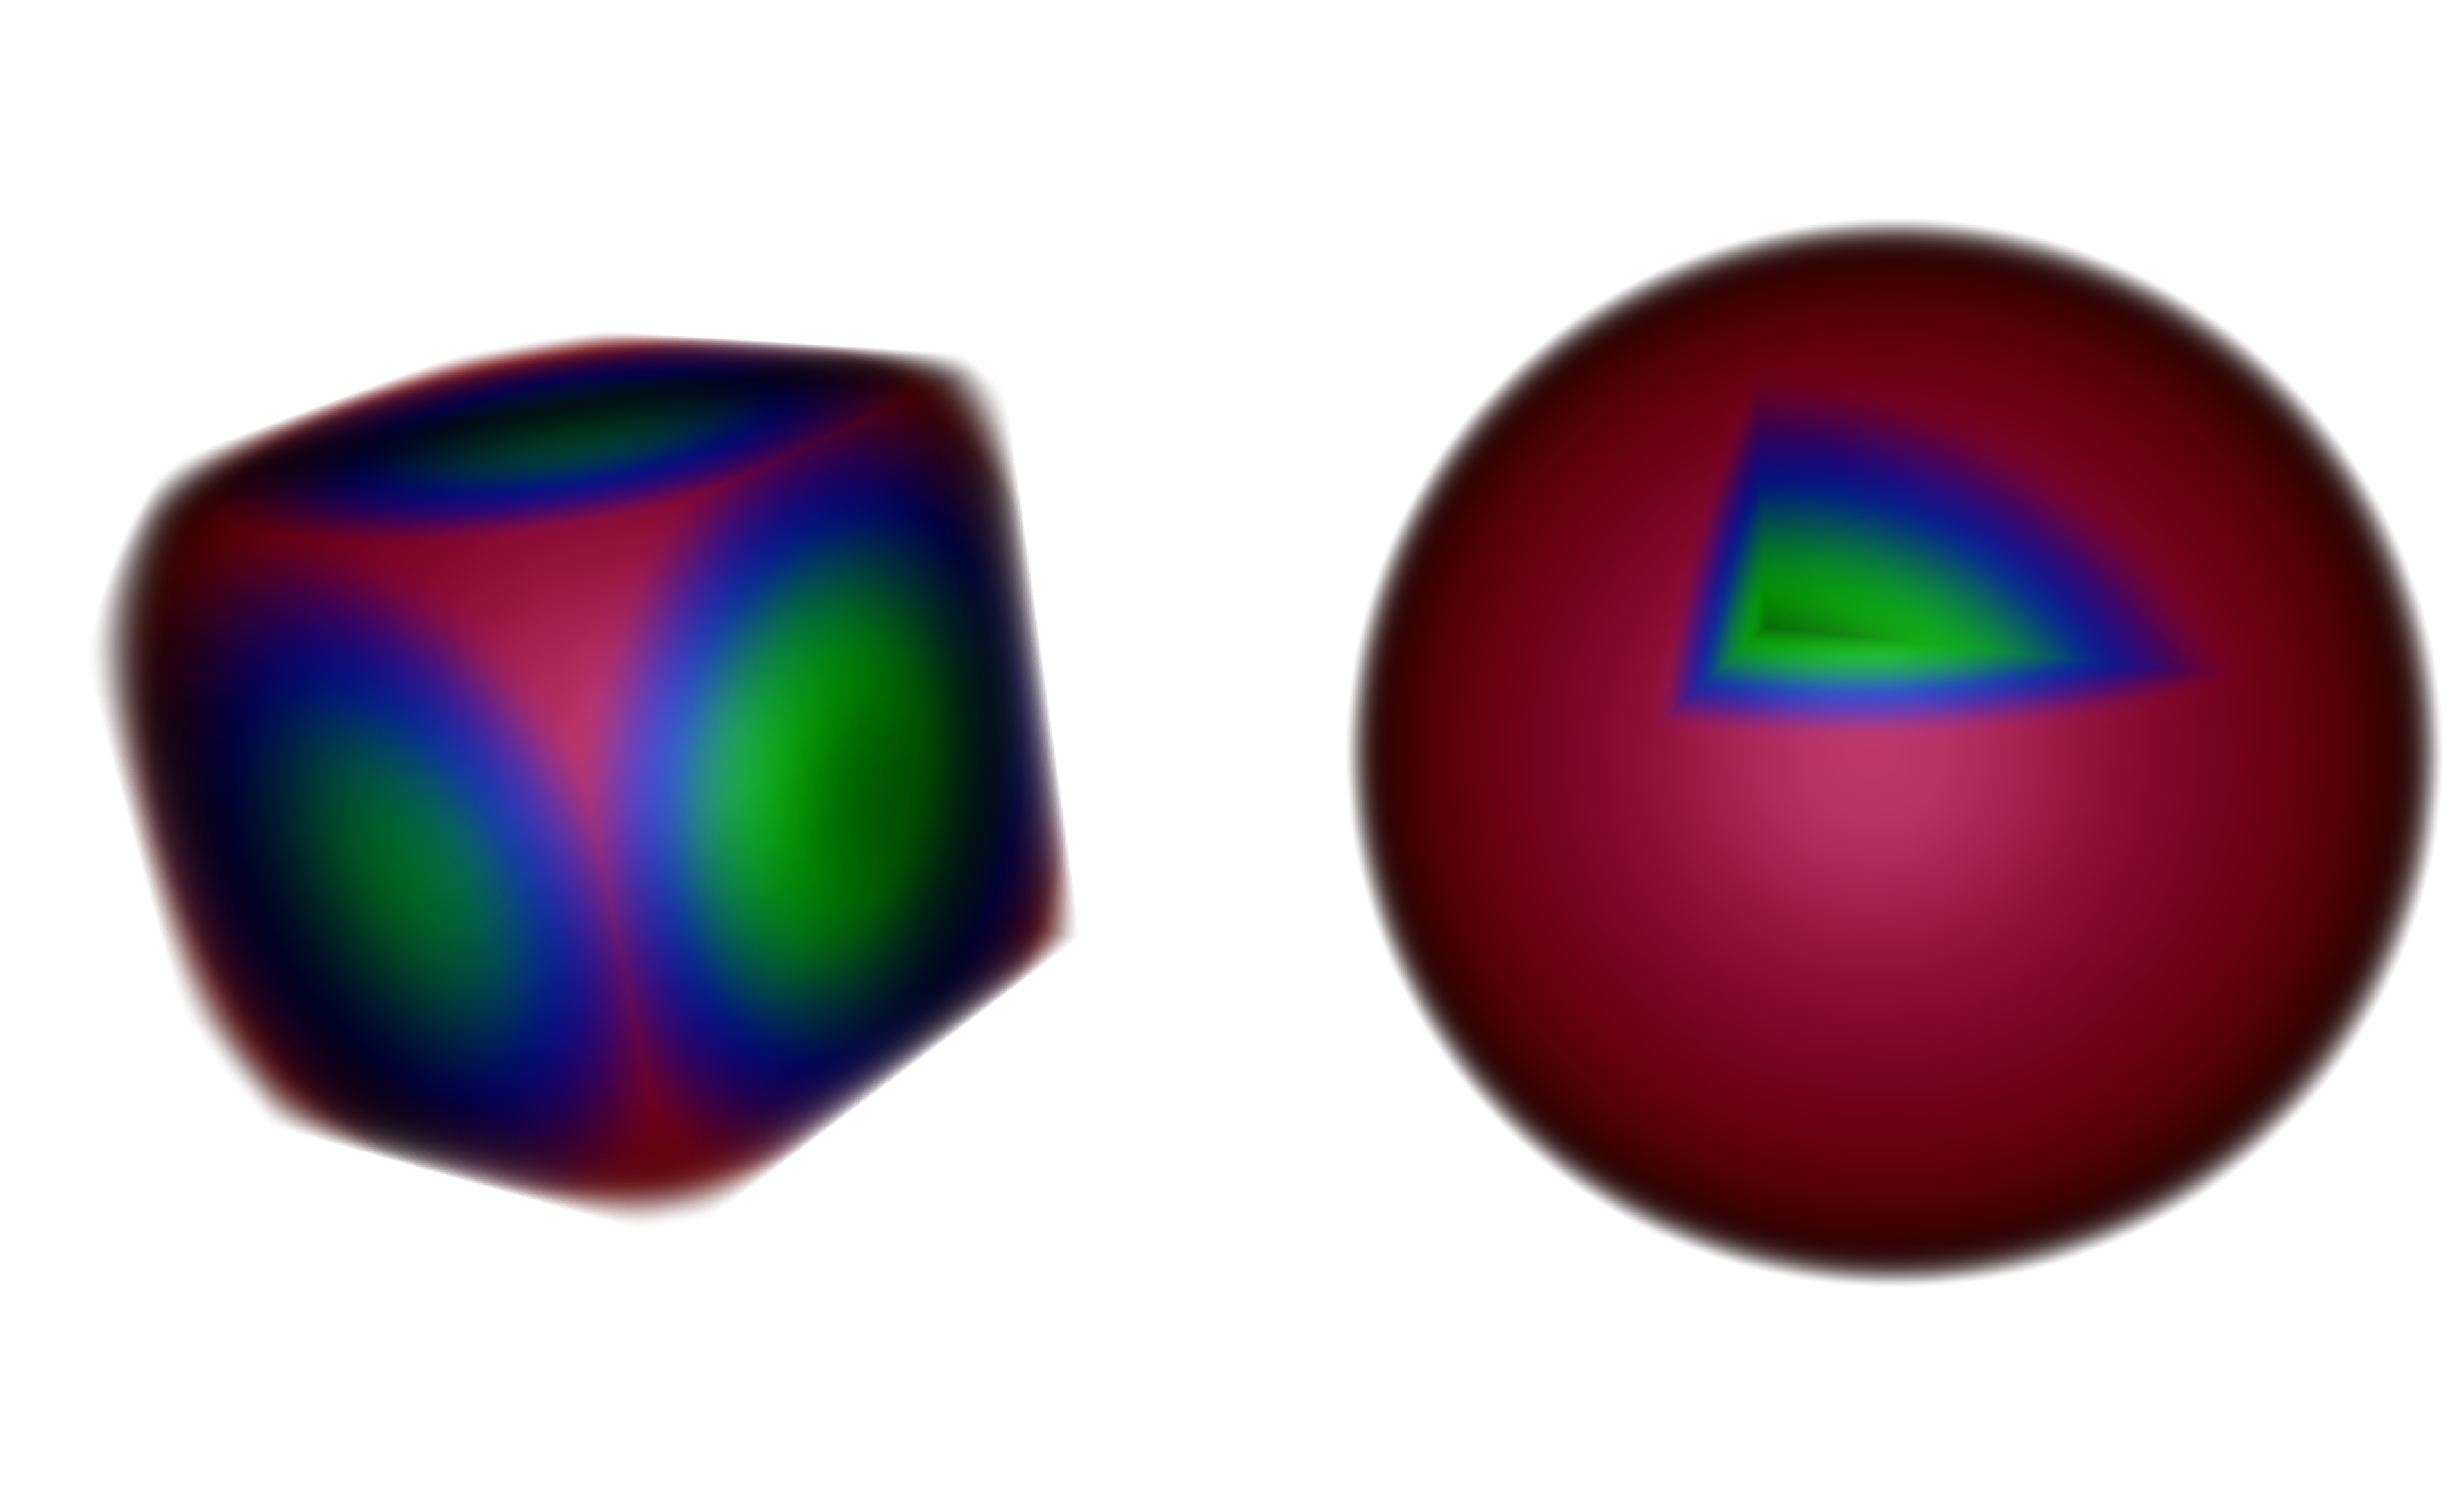
\includegraphics[width=2.5in]{SphereCropping.png}
  \caption{A sphere is cropped using two different configurations of cropping regions.}
  \label{fig:cropping}
\end{figure}

\subsection{Wide Support of Data Types}
The mapper supports most signed and unsigned data types such as short, int,
float and double as well as the two most common data abstractions in VTK,
cell and point data.  Bias and scale factors are pre-computed and passed into
the fragment shader to normalize the data values for correct look-up table
mapping.

\begin{figure}[ht]
  \centering
  \begin{subfigure}[b]{.5\columnwidth}
    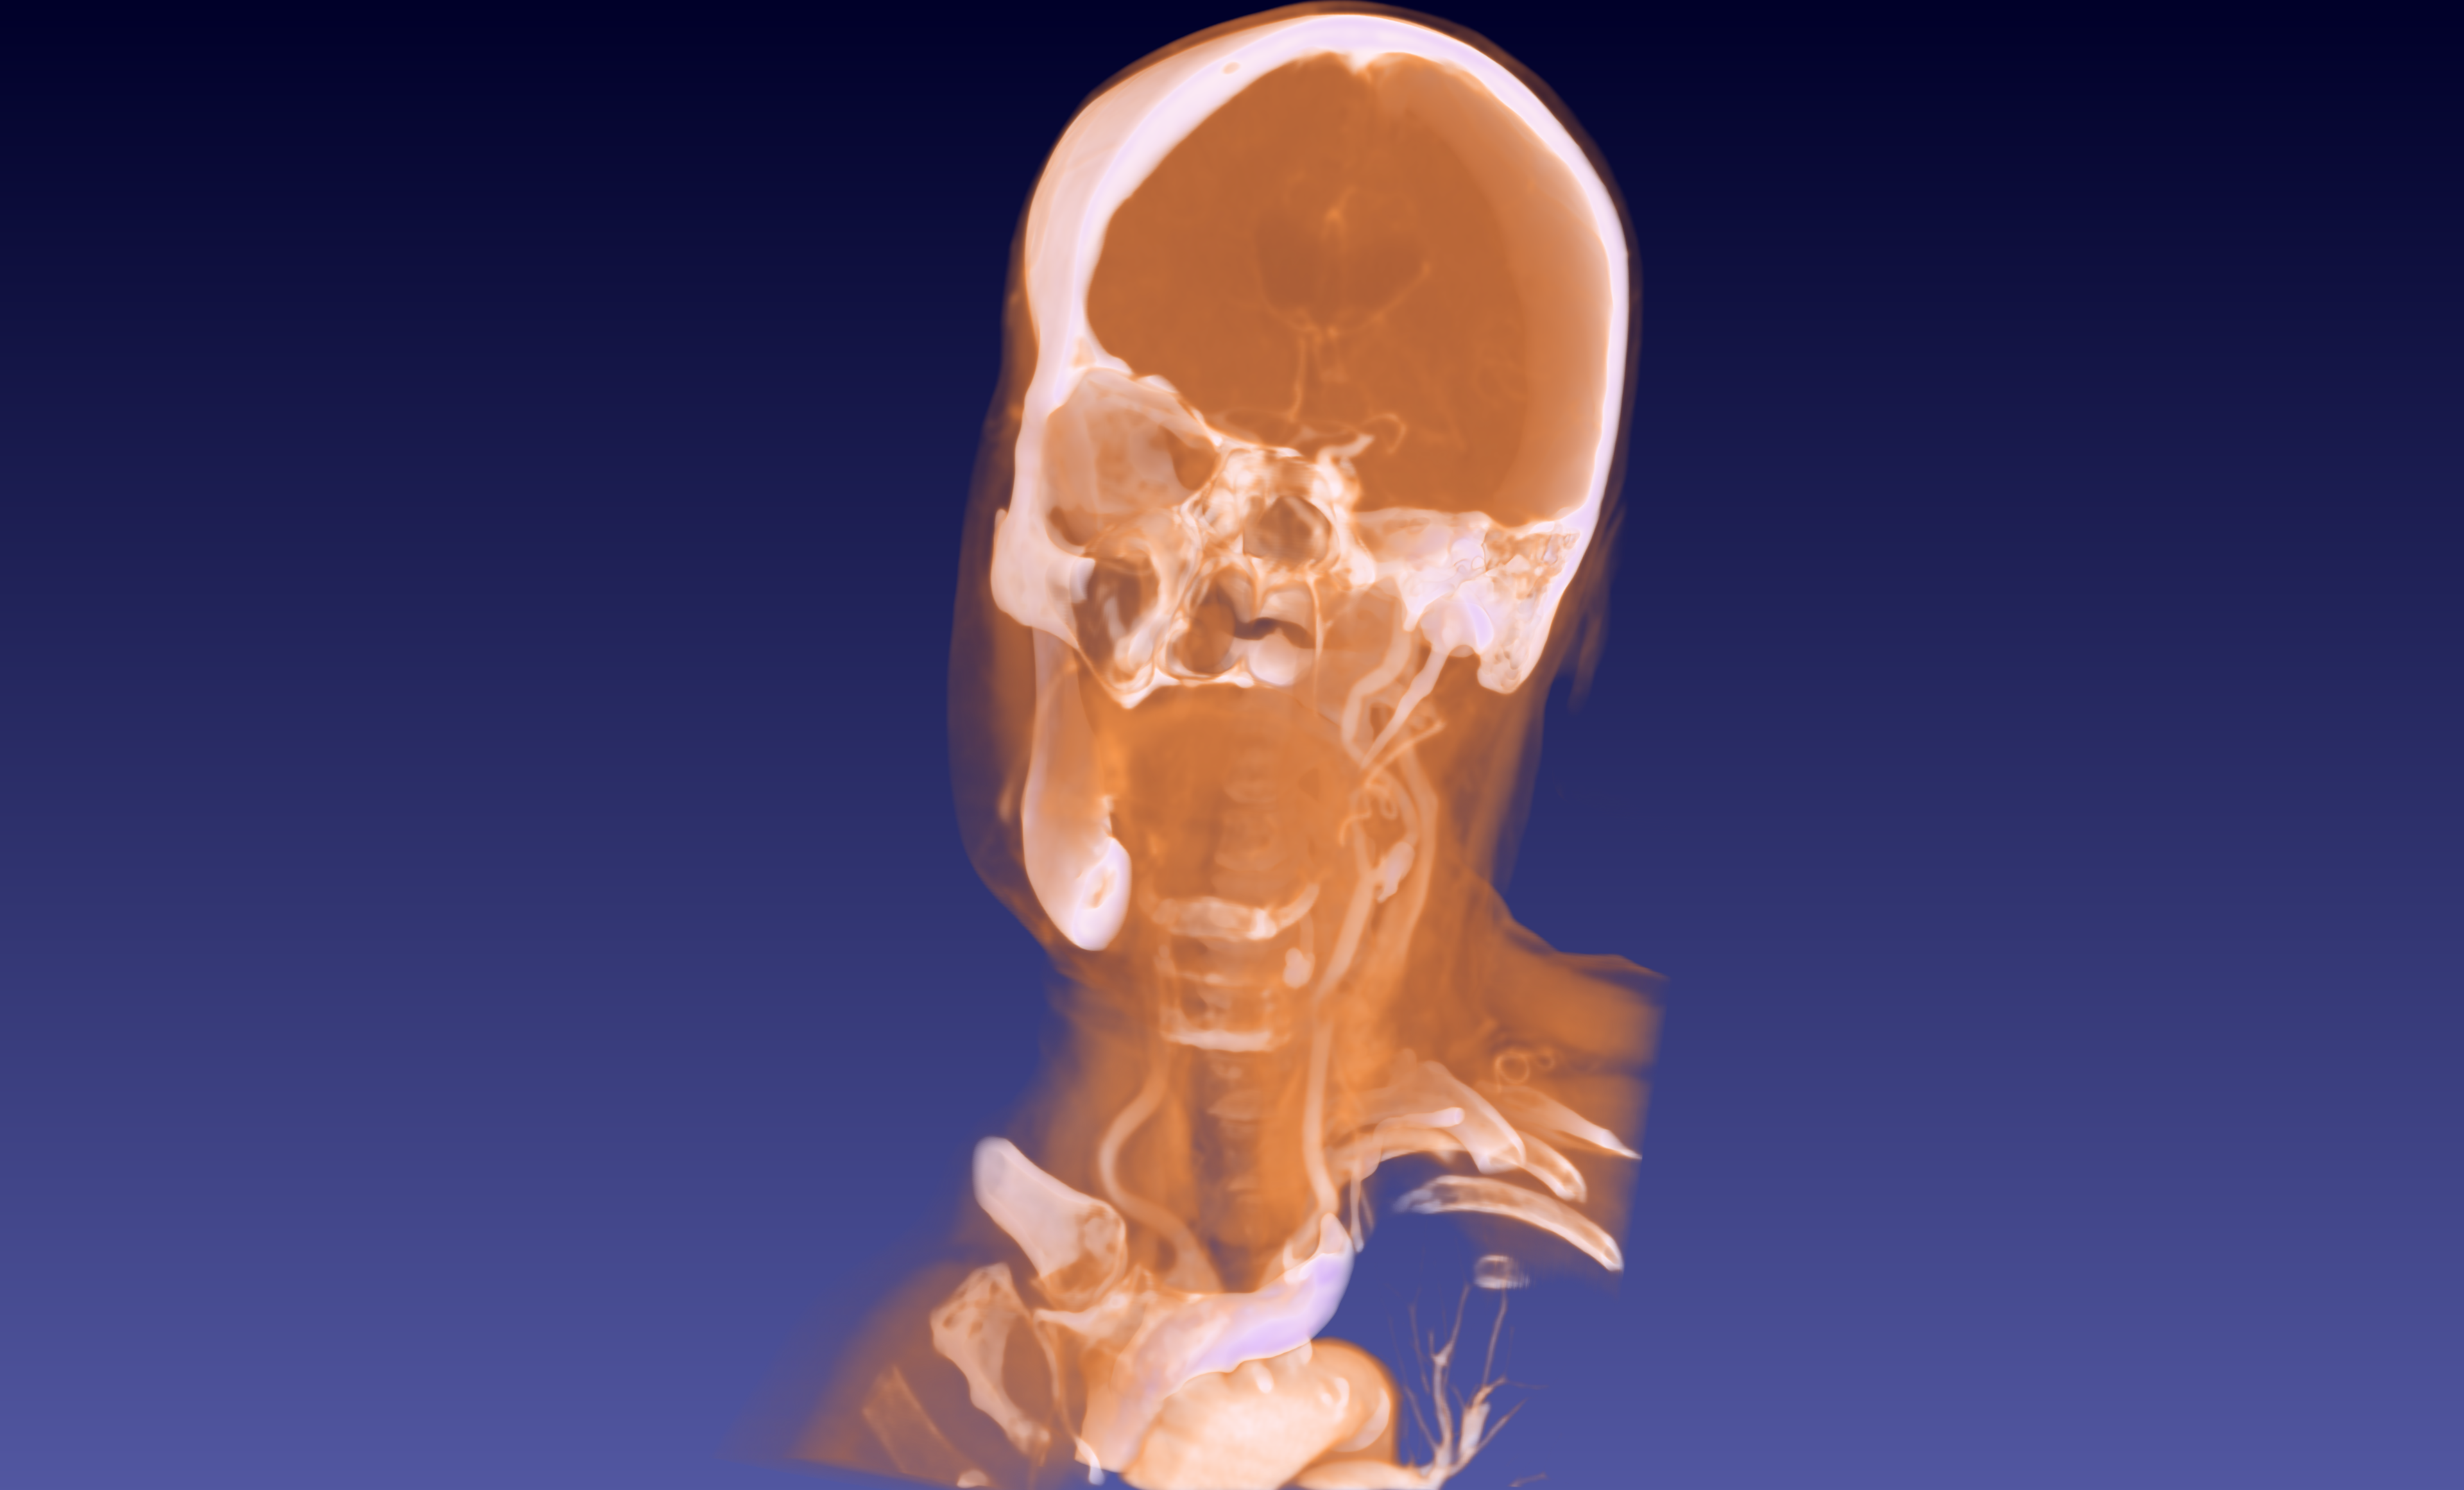
\includegraphics[width=\textwidth]{HeadClippingSlabNoShading.png}
    \caption{Without shading}
    \label{fig:clipnoshading}
  \end{subfigure}%
  \begin{subfigure}[b]{.5\columnwidth}
    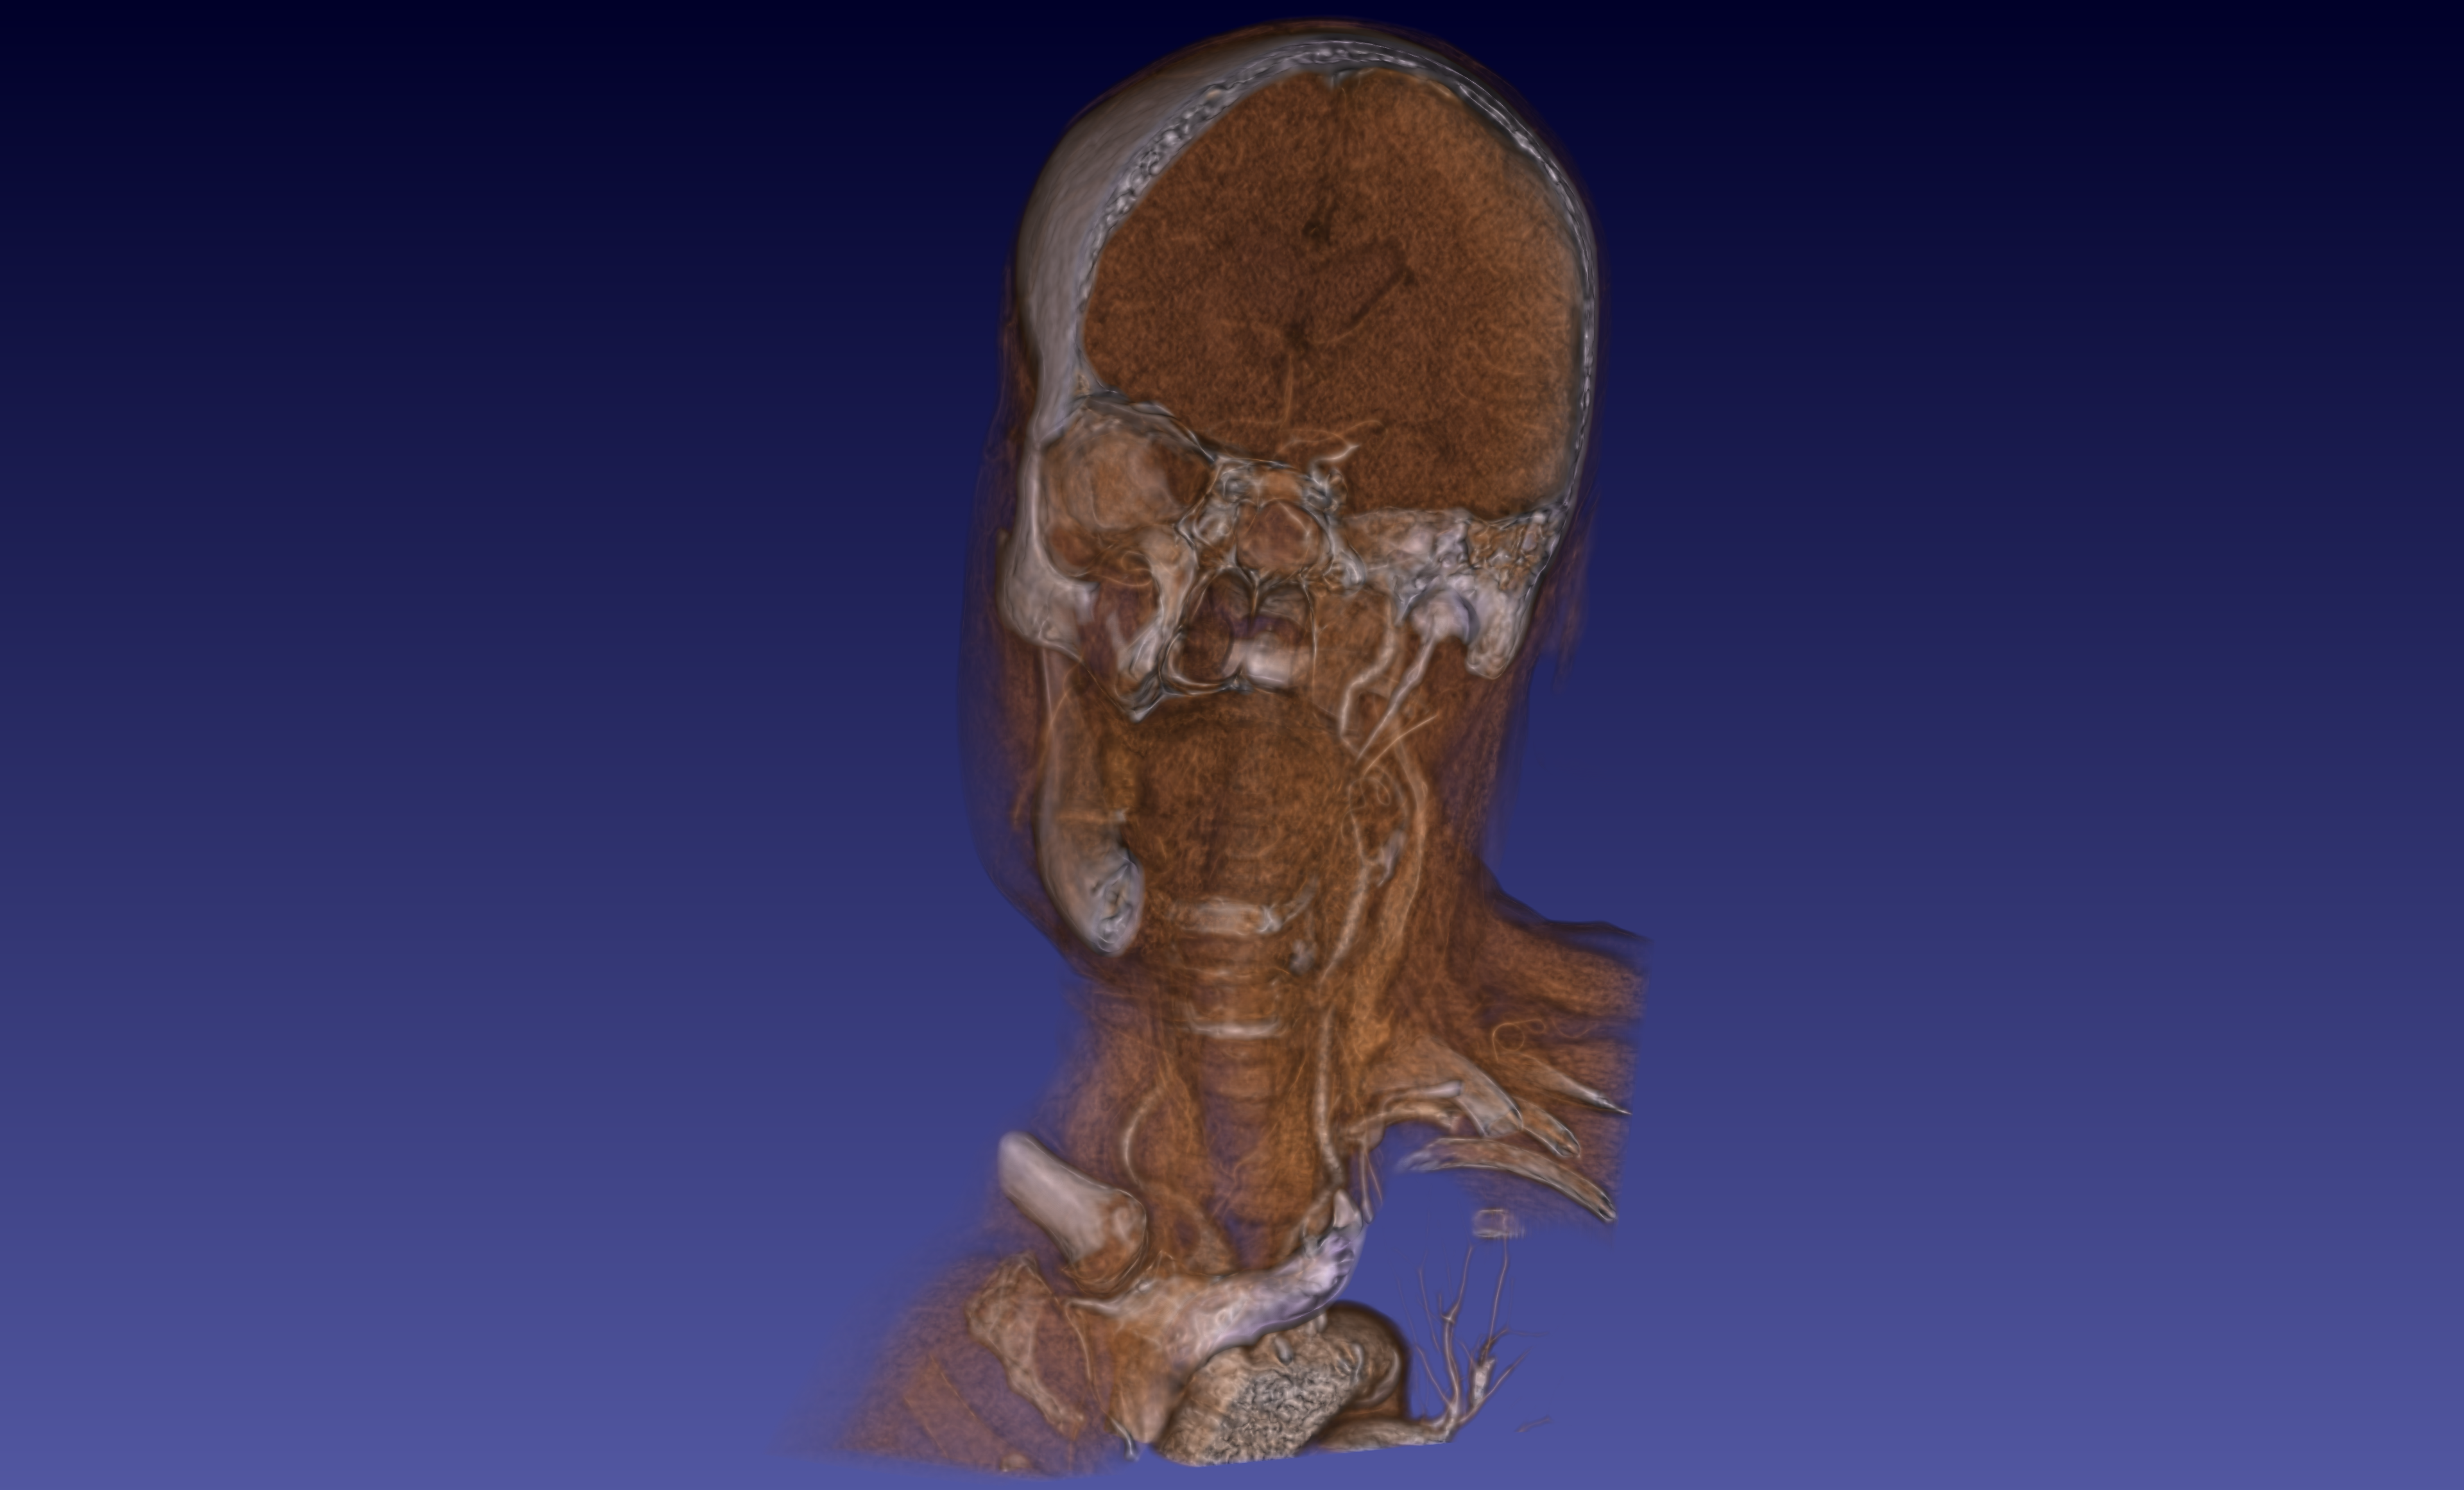
\includegraphics[width=\textwidth]{HeadClippingSlabShading.png}
    \caption{With shading}
    \label{fig:clipshading}
  \end{subfigure}%
  \caption{A pair of parallel clipping planes clip the volume}
  \label{fig:clipping}
\end{figure}

\subsection{Blending Modes}
The mapper supports composite blending, minimum intensity projection, maximum
intensity projection, additive intensity and average intensity blending. Each of
these blending modes are useful for a particular use-case in medical computing.
The most common one which is also the default is the composite blending mode.
See Figure~\ref{fig:blendingmodes} for an example of the different blend modes
on the same data.

\begin{figure}[htbp]
  \centering
  \begin{subfigure}{.5\columnwidth}
    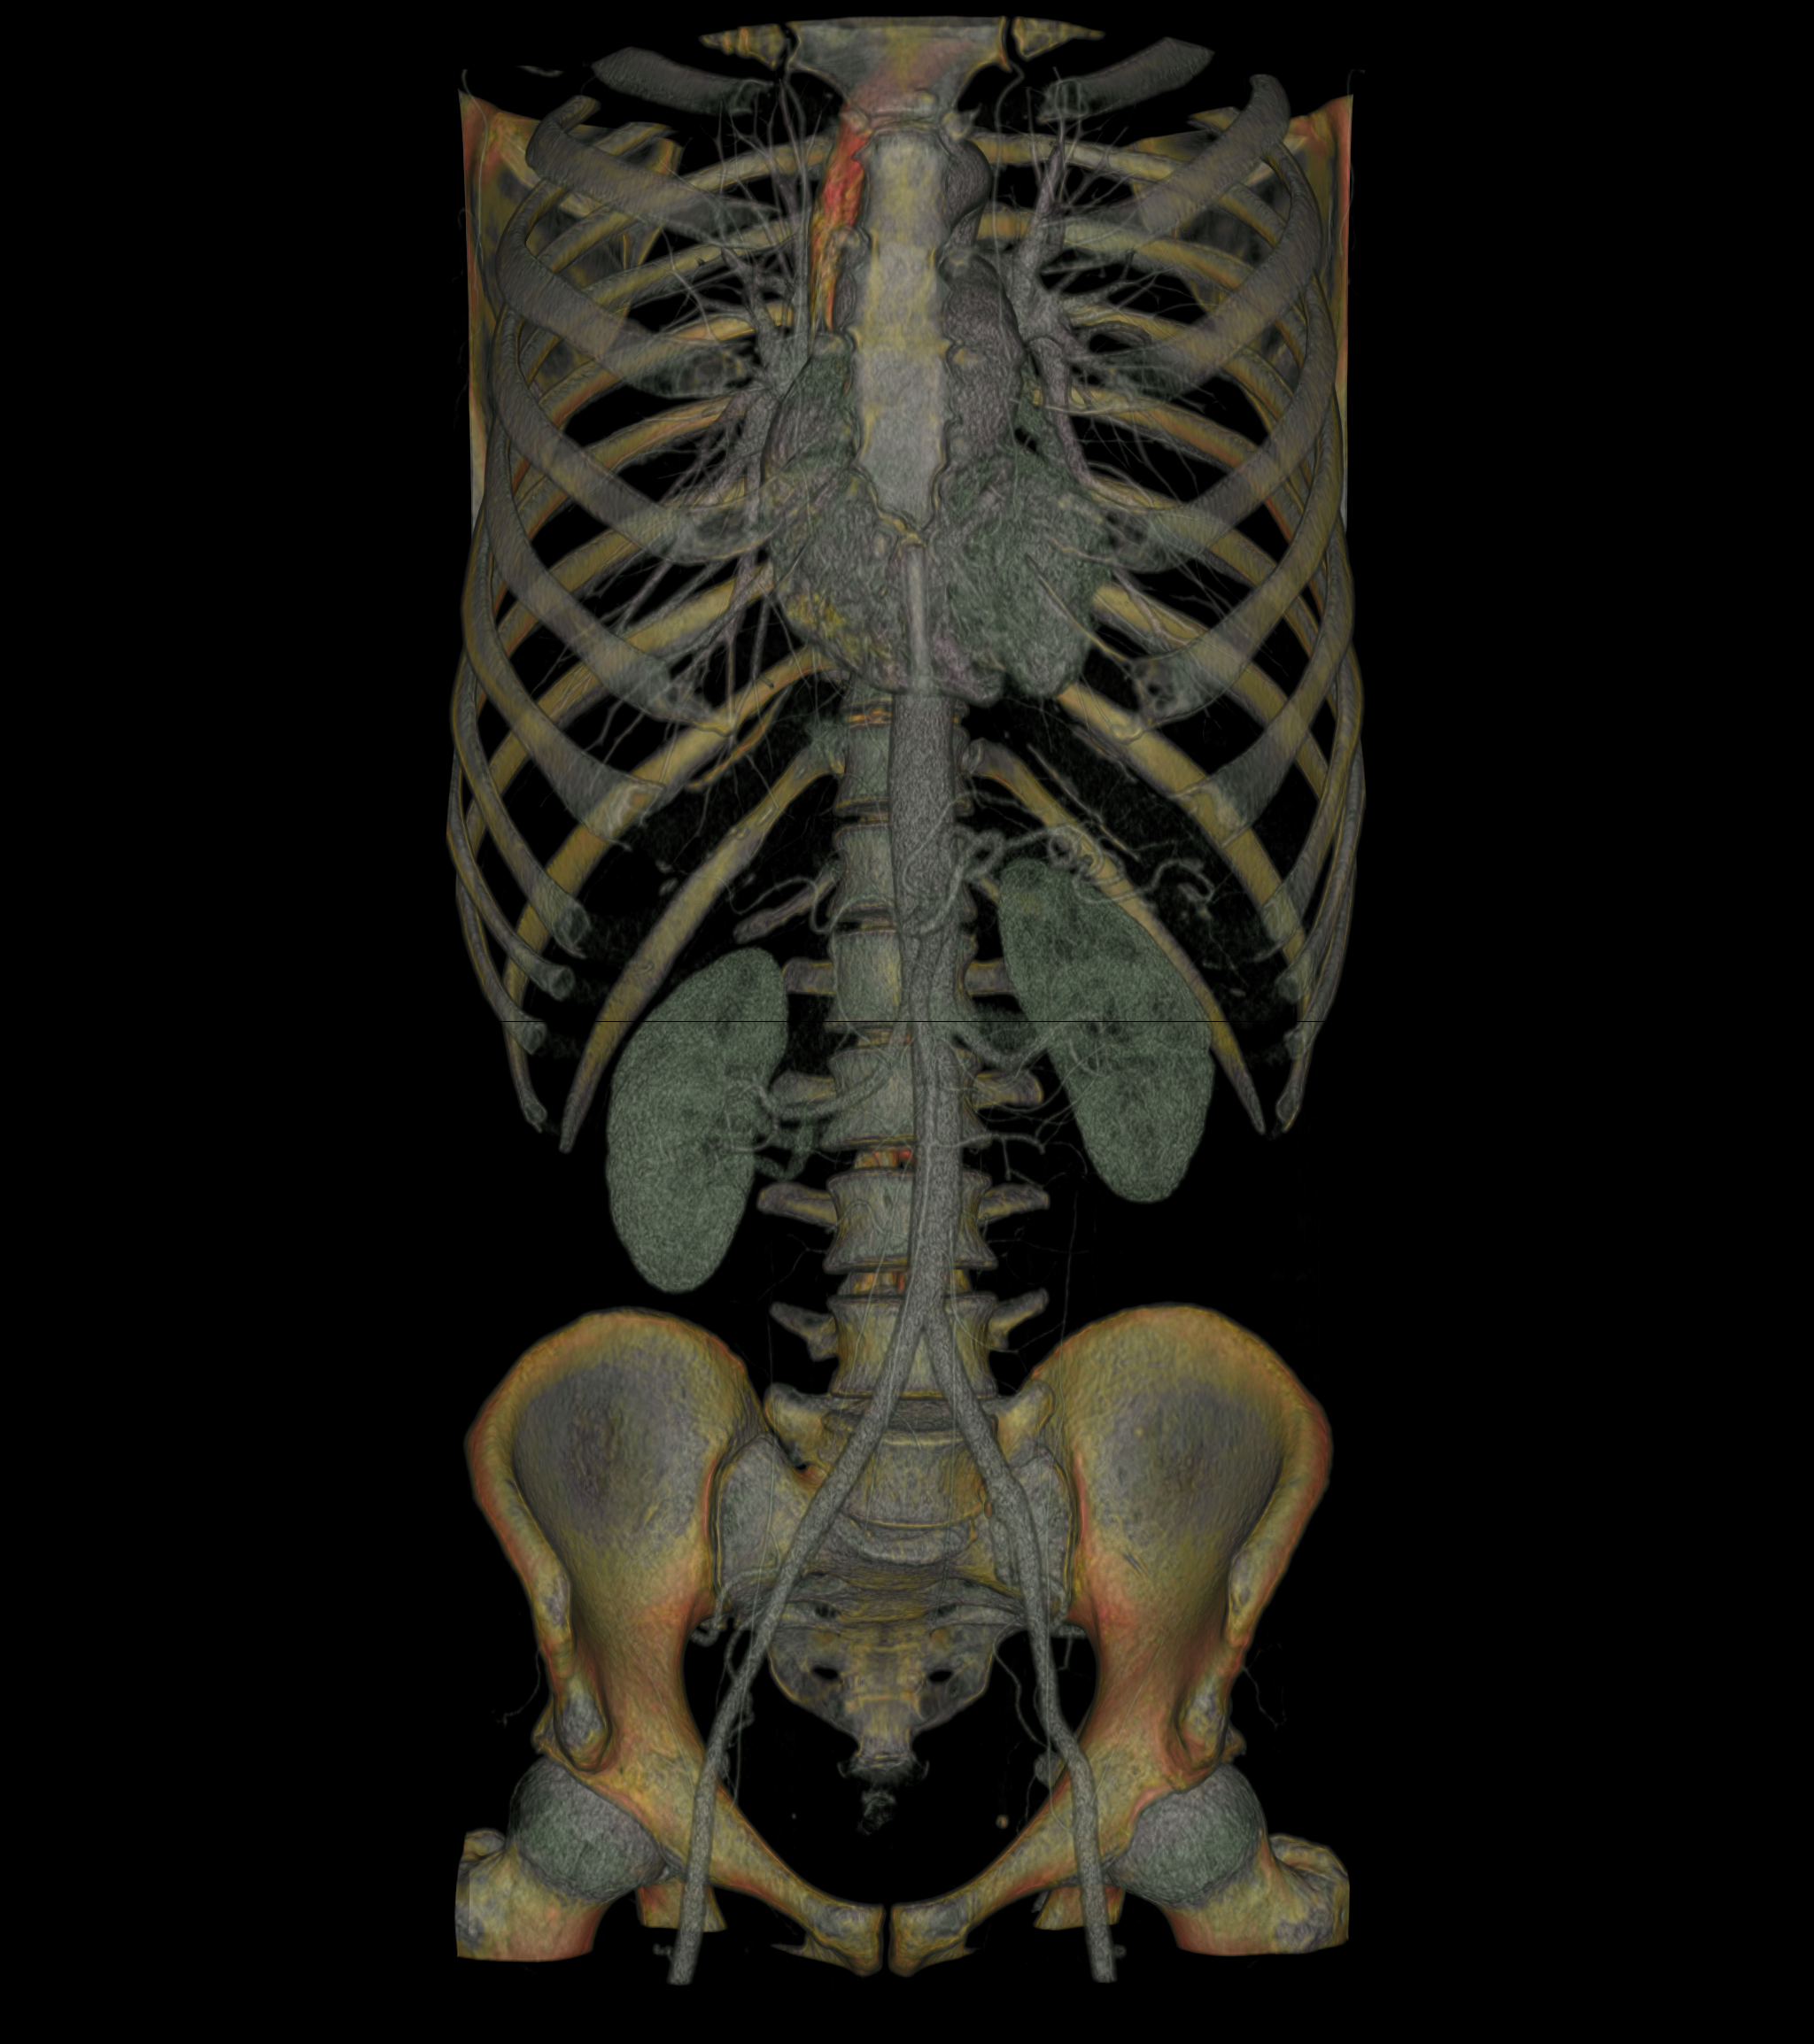
\includegraphics[width=\columnwidth]{TorsoBlendingComposite.png}
    \caption{Composite}
    \label{fig:blendcomposite}
  \end{subfigure}%
  \begin{subfigure}{.5\columnwidth}
    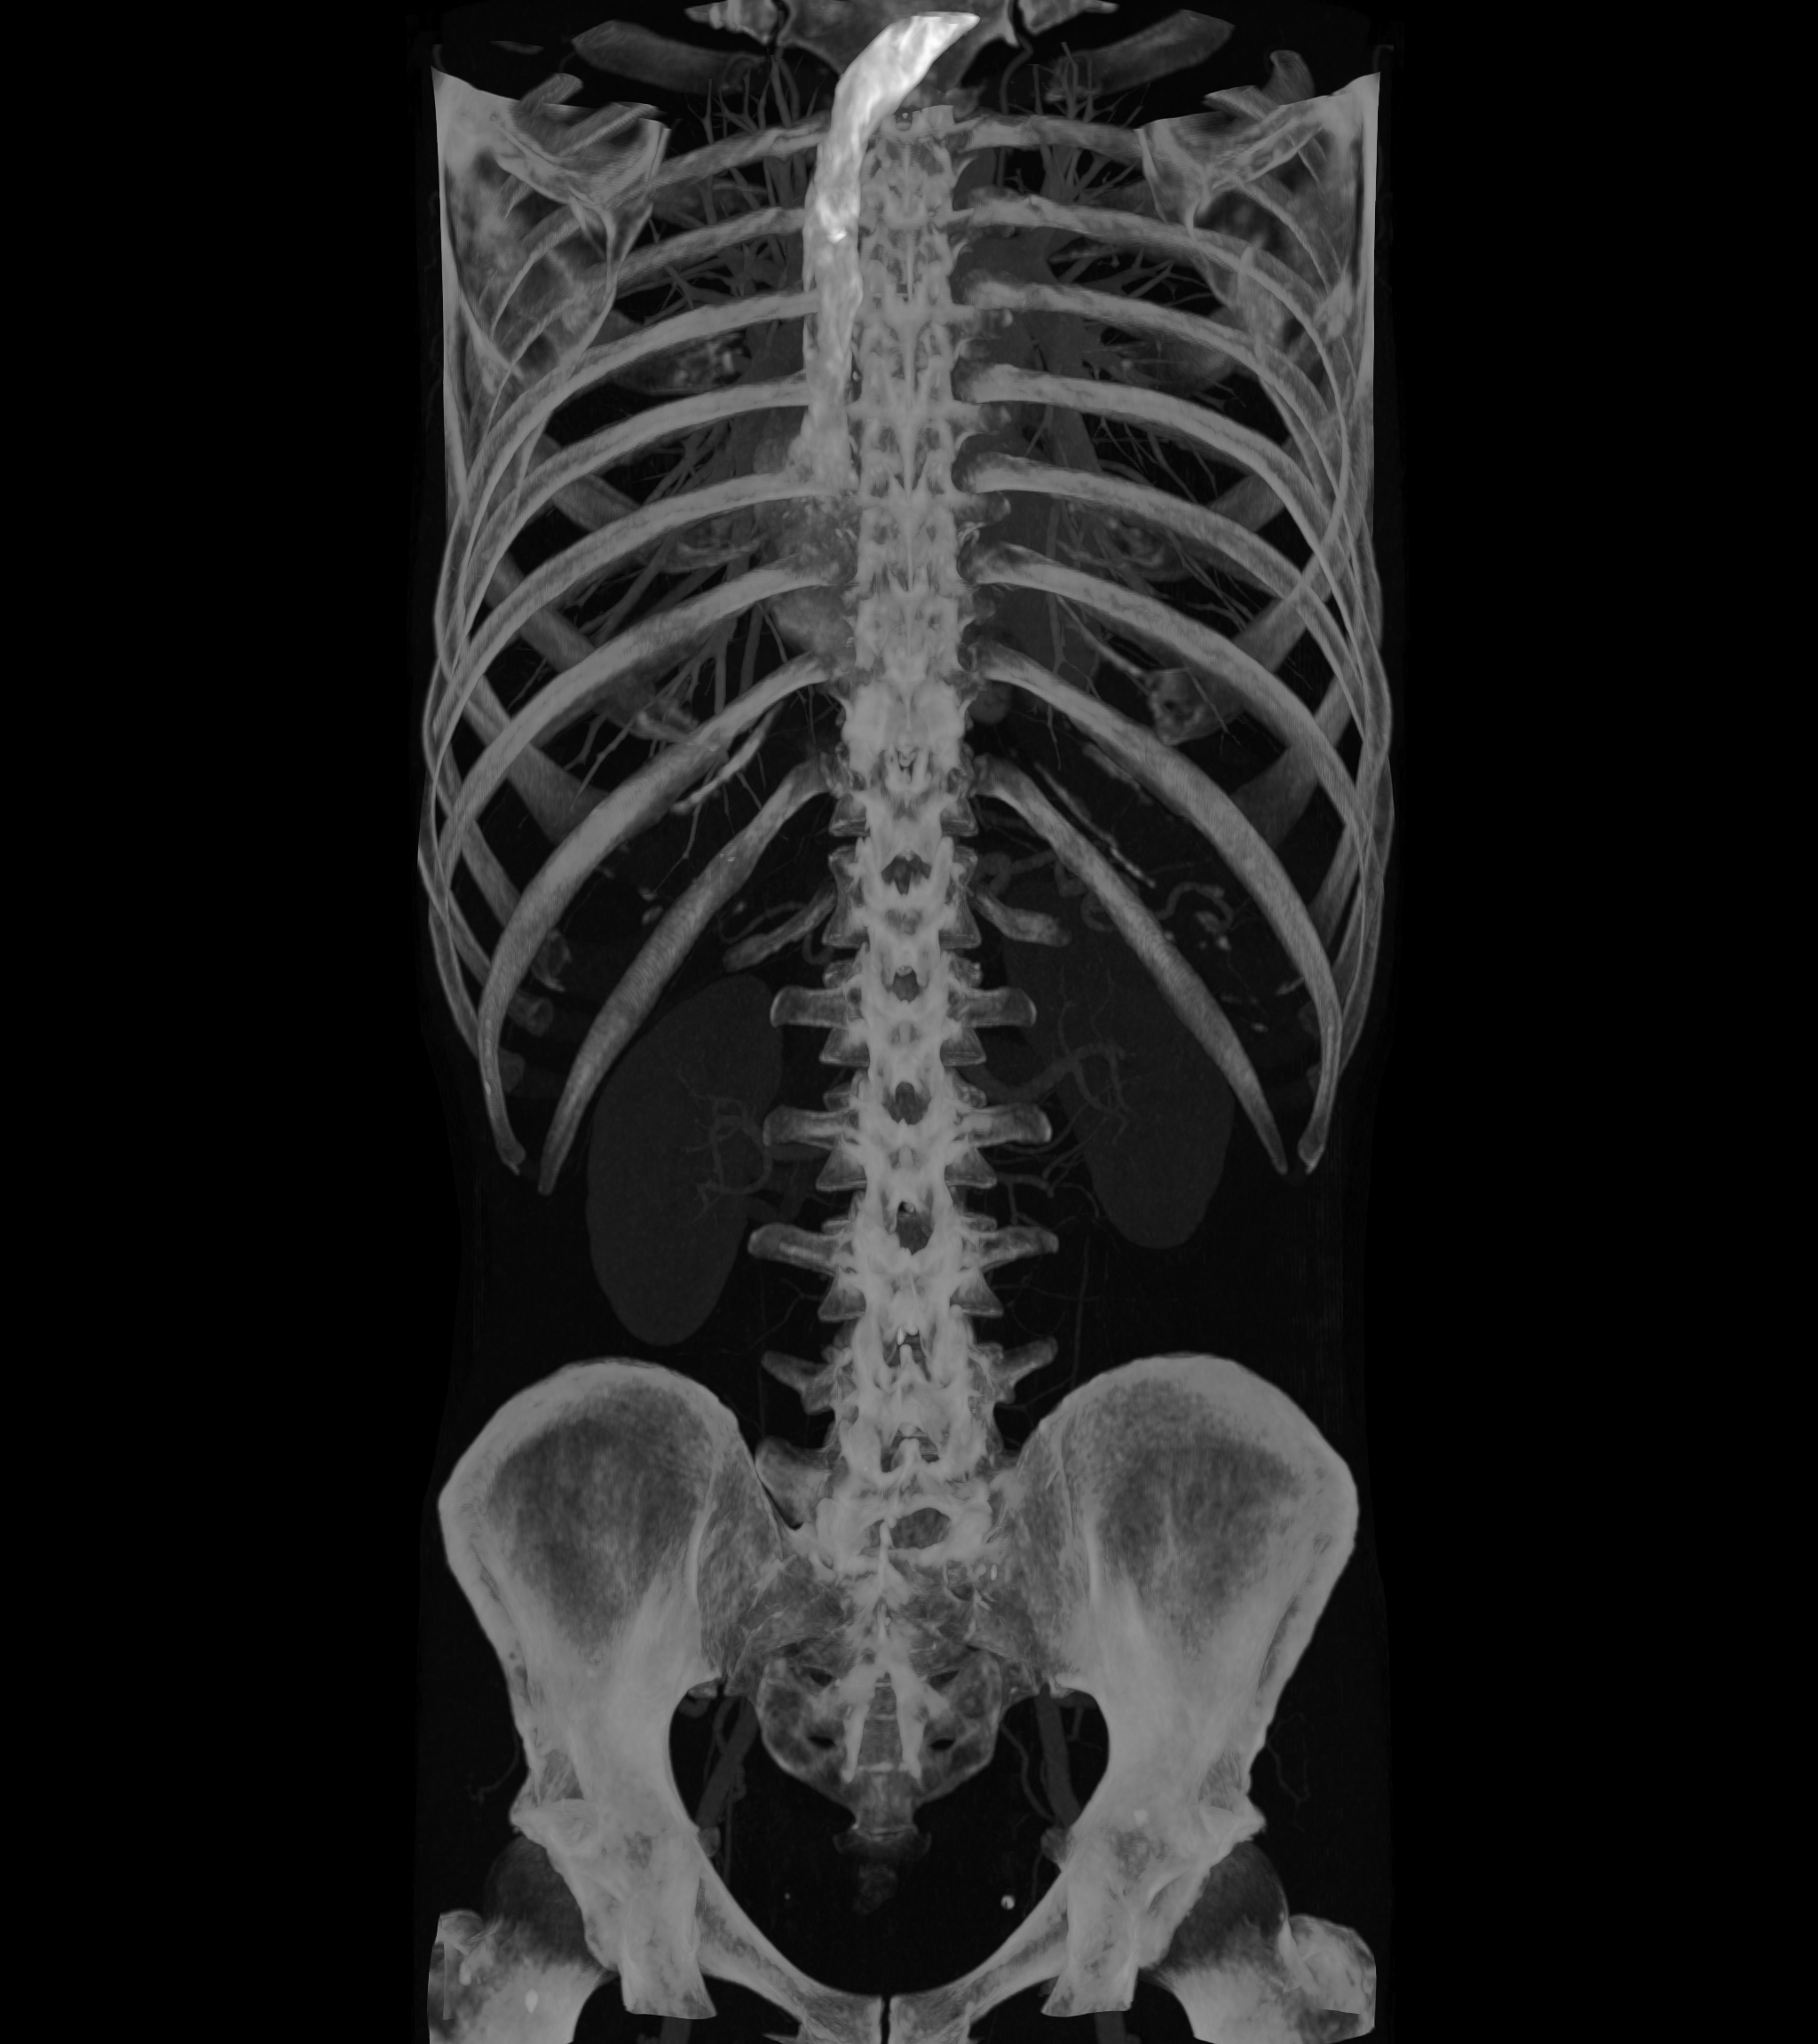
\includegraphics[width=\columnwidth]{TorsoBlendingMIP.png}
    \caption{Maximum Intensity}
    \label{fig:blendmax}
  \end{subfigure}
  \begin{subfigure}{.5\columnwidth}   
    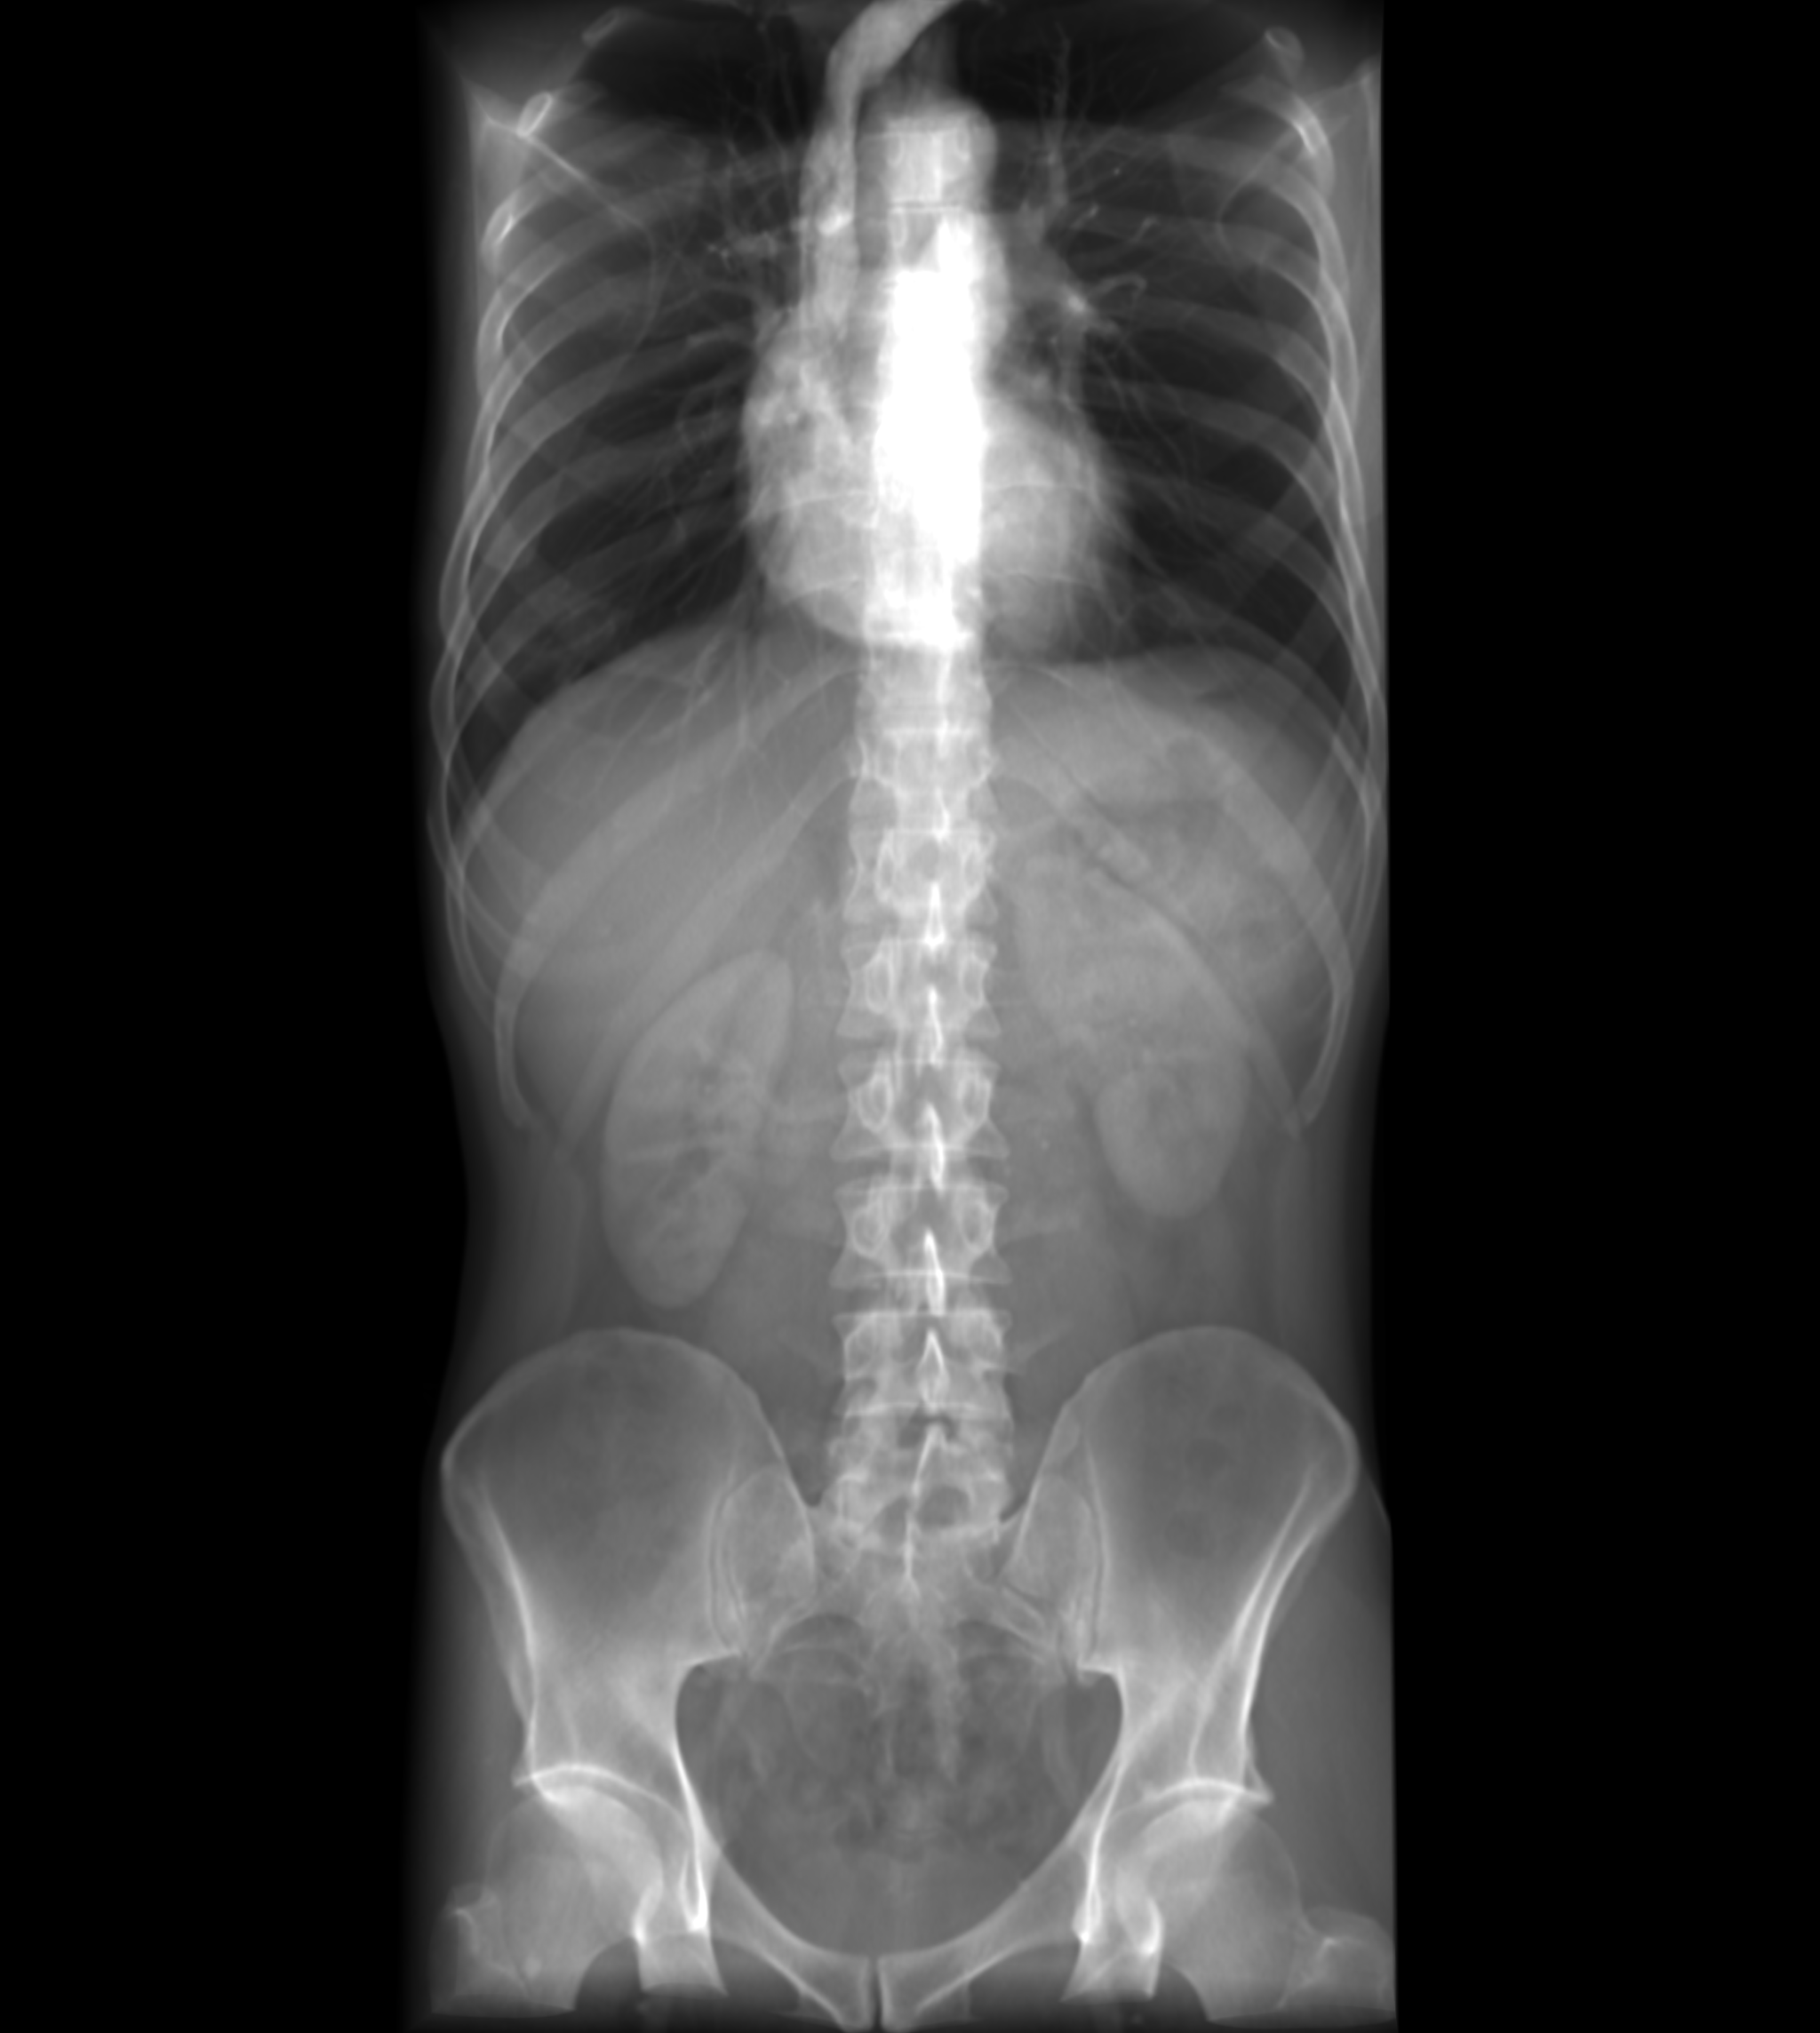
\includegraphics[width=\columnwidth]{TorsoBlendingAdditive.png}
    \caption{Additive}
    \label{fig:blendadditive}
  \end{subfigure}%
  \begin{subfigure}{.5\columnwidth}
    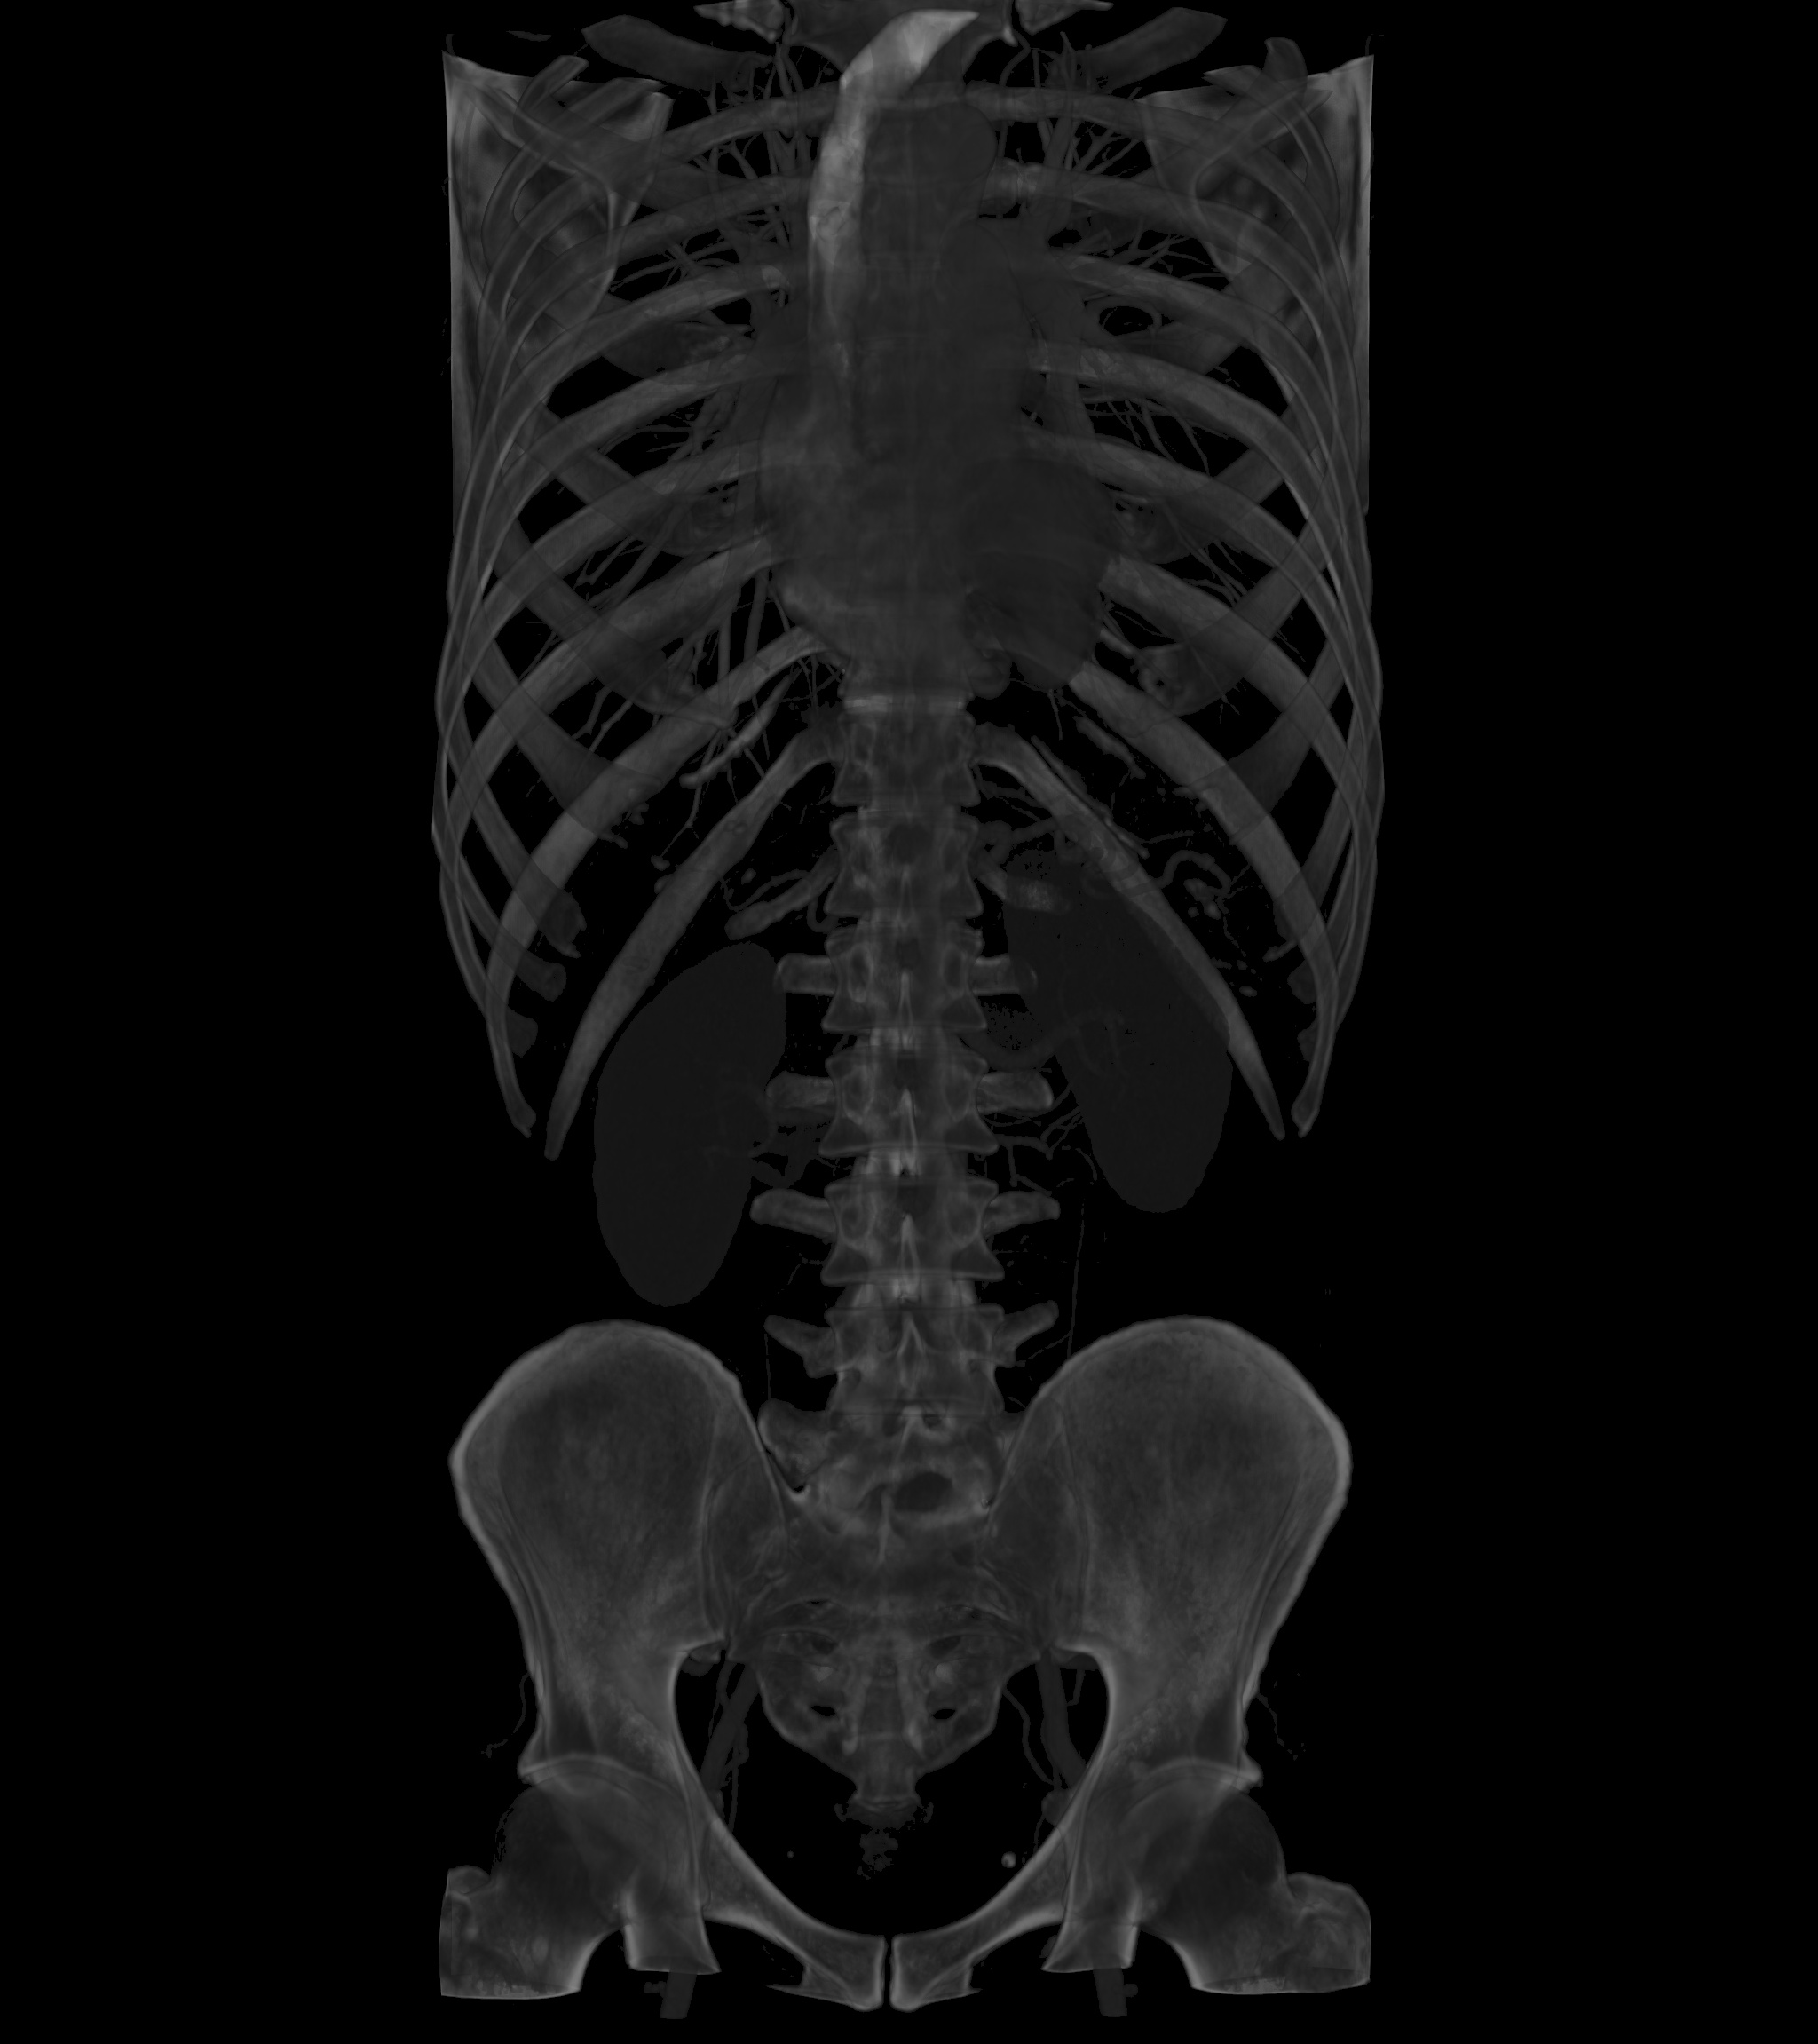
\includegraphics[width=\columnwidth]{TorsoBlendingAverage.png}
    \caption{Average Intensity}
    \label{fig:blendaverage}
  \end{subfigure}
  \caption{Blend modes supported by the \texttt{vtkGPUVolumeRayCastMapper}}
  \label{fig:blendingmodes}
\end{figure}

\subsection{Masking}
Both binary and label masks are supported. With binary masks, the value in the
masking volume indicates visibility of the voxel in the data volume. When a
label map is in use, the value in the label map is used to select different
rendering parameters for that sample.  See Figure 5 for an example of label data
masks.

\subsection{Opacity Modulated by Gradient Magnitude} A transfer function
mapping the magnitude of the gradient to an opacity modulation value can be used
to essentially perform edge detection (de-emphasize homogenous regions) during
rendering. See ~\ref{fig:gradient} for an example of rendering with and without
the use of a gradient opacity transfer function.

\begin{figure}[ht]
  \centering
   \begin{subfigure}[b]{0.5\columnwidth}
     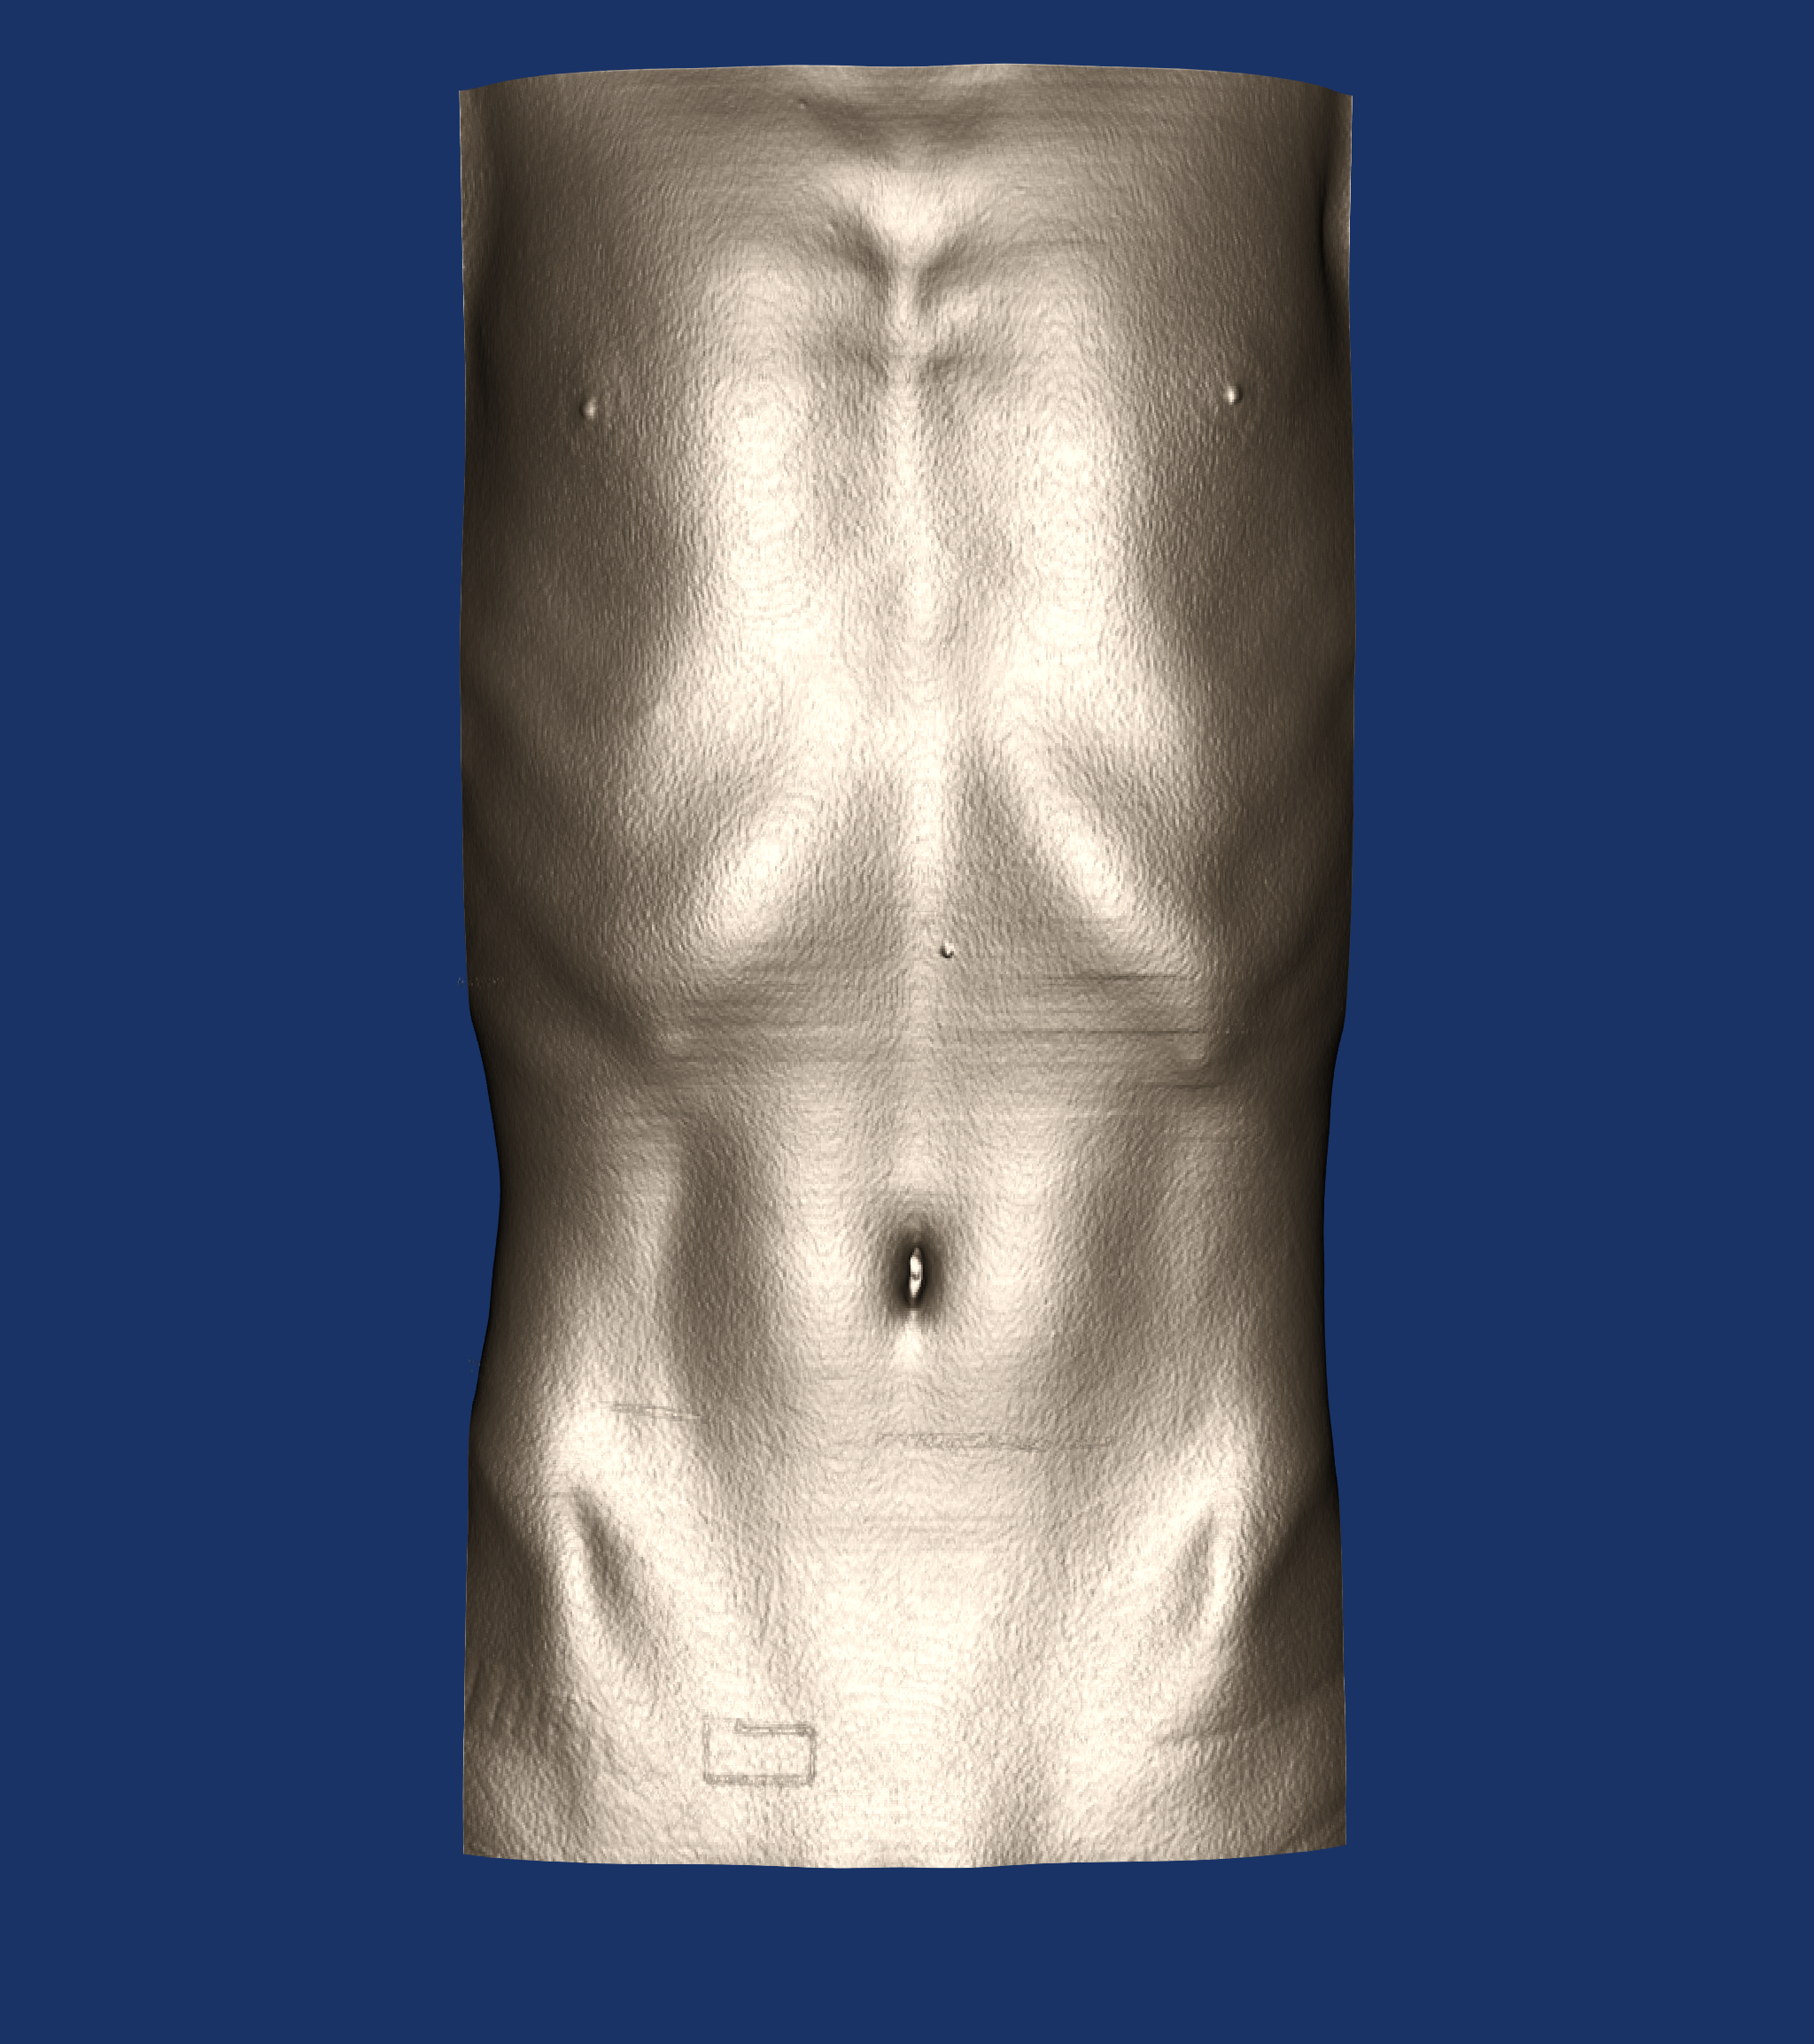
\includegraphics[width=\columnwidth]{TorsoNoGradient.png}
     \caption{Without gradient opacity function}
     \label{fig:Ng1} 
   \end{subfigure}%
  \begin{subfigure}[b]{0.5\columnwidth}
    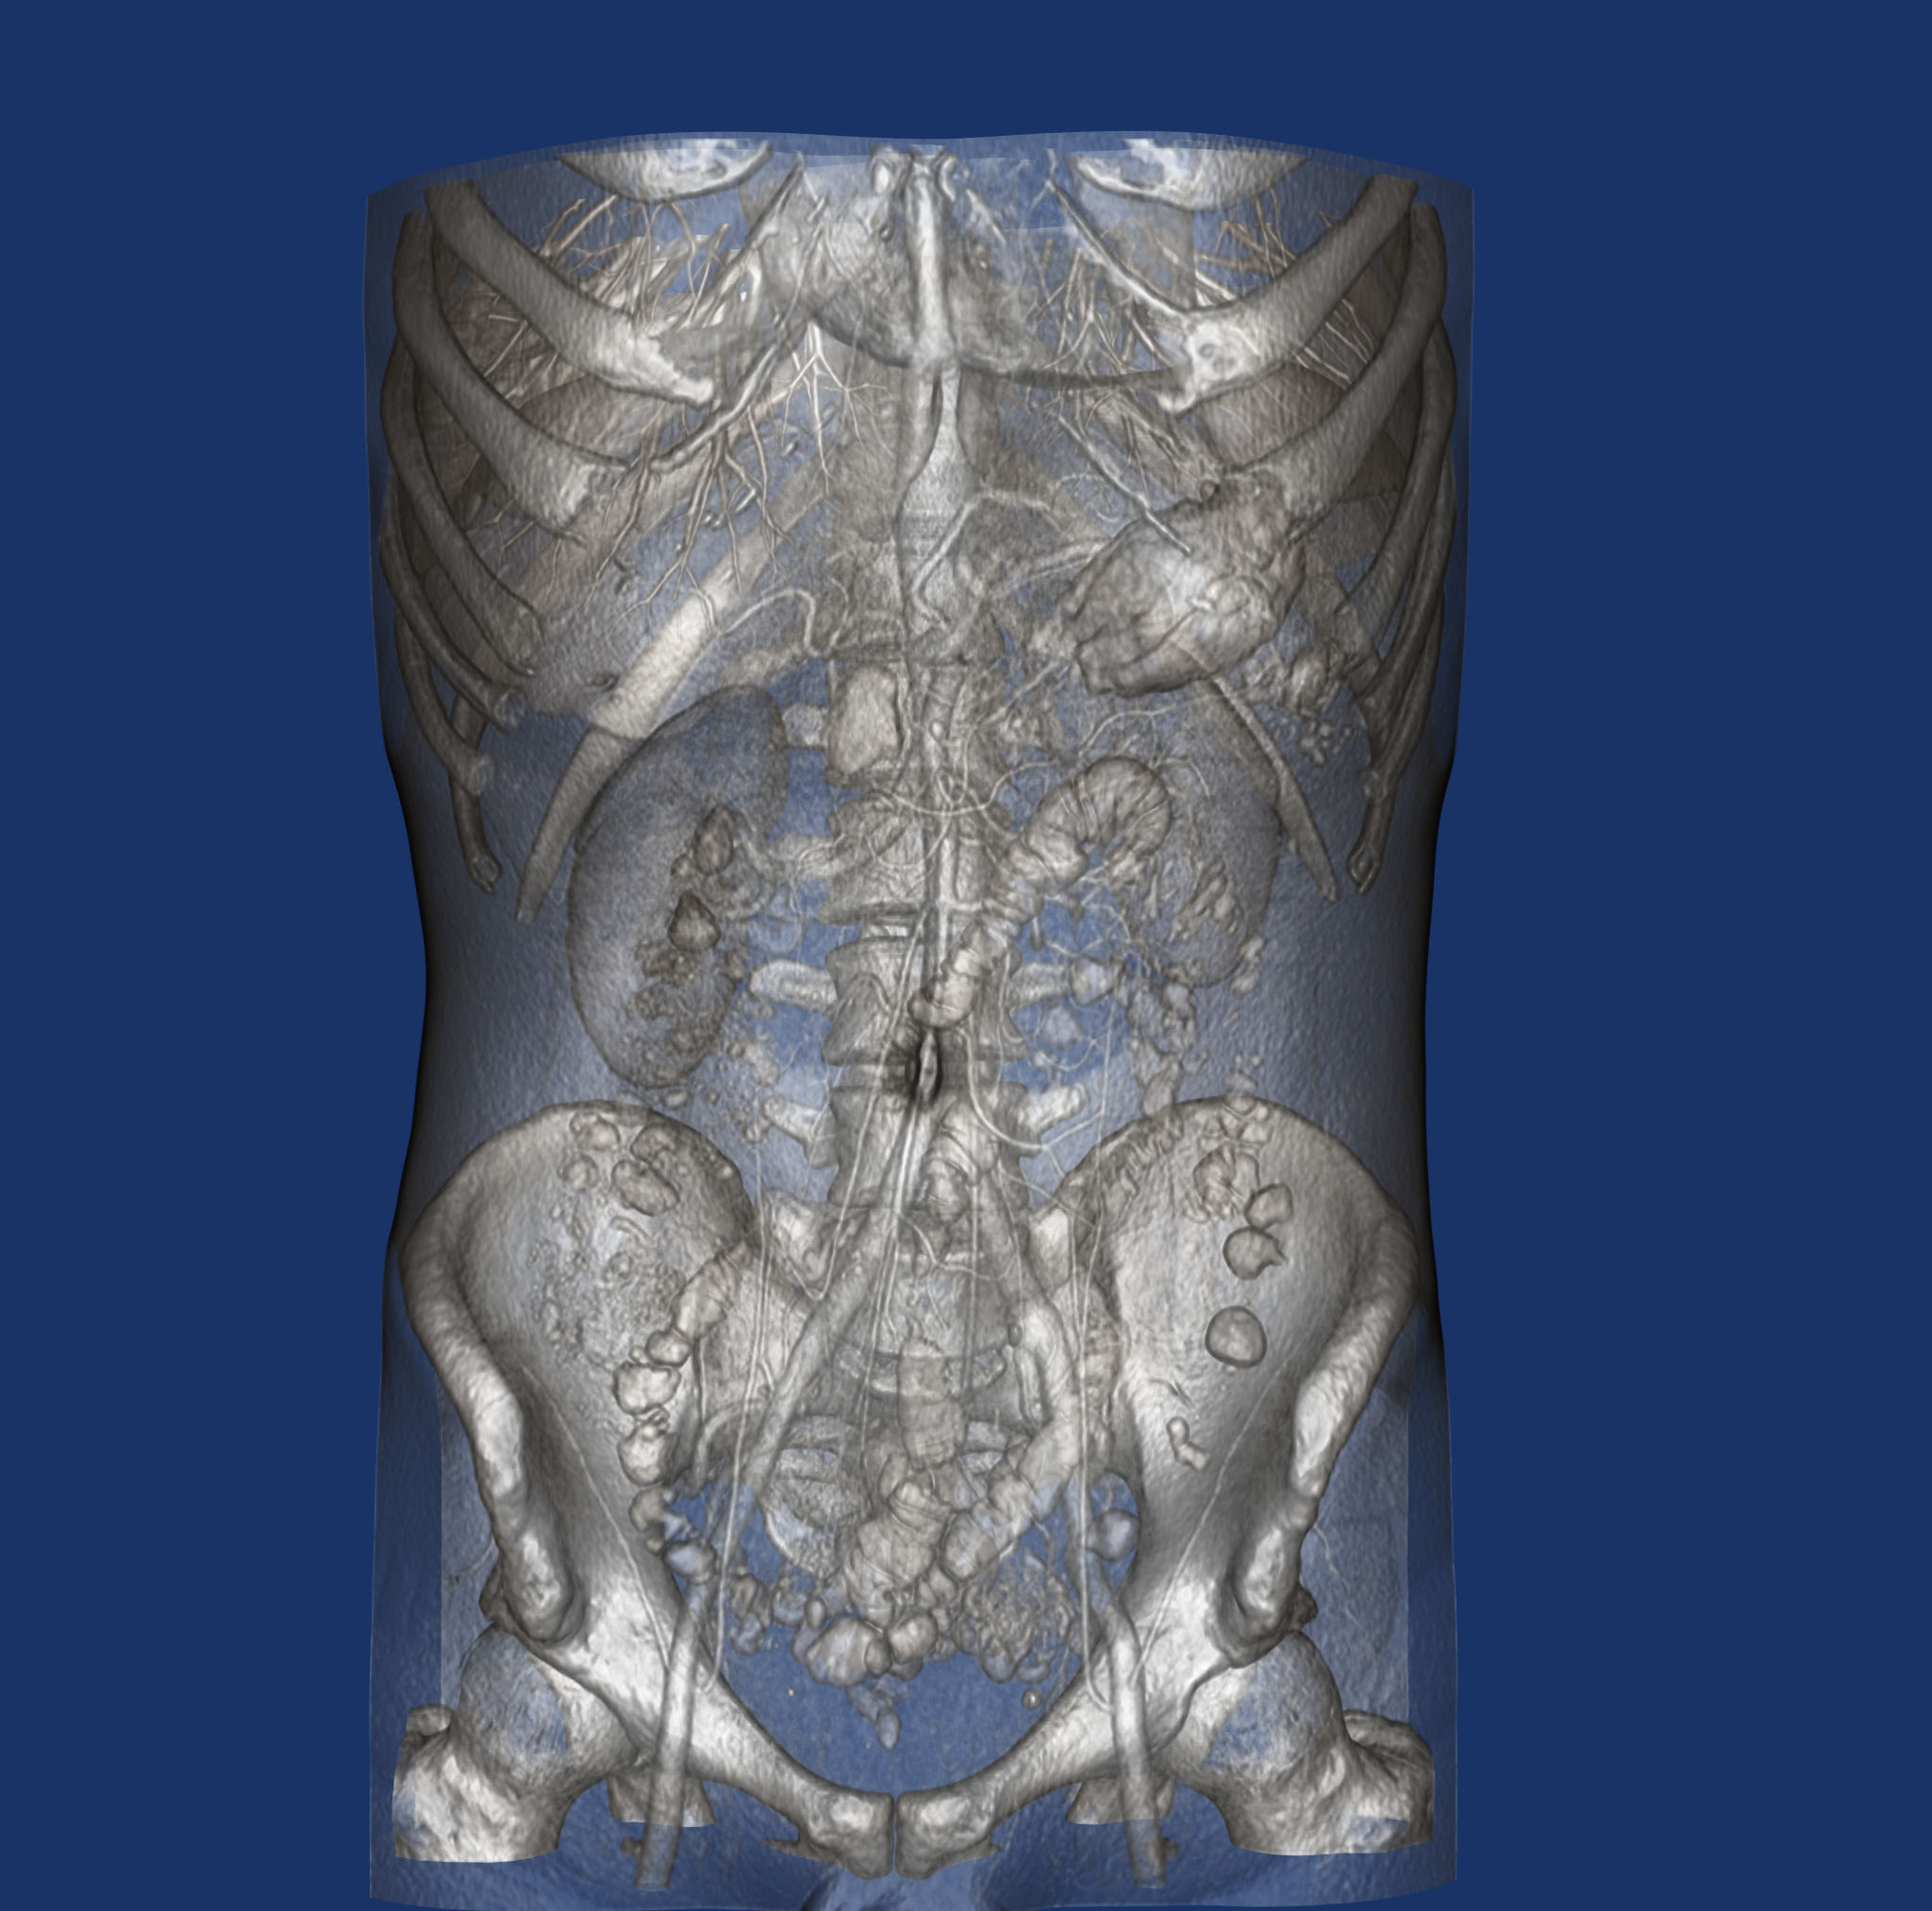
\includegraphics[width=\columnwidth]{TorsoGradient.png}
    \caption{With gradient opacity function}
    \label{fig:Ng2}
  \end{subfigure}
  \caption{Gradient magnitude based opacity modulation}
  \label{fig:gradient}
\end{figure}

\begin{figure}[ht]
  \centering
  \includegraphics[width=\columnwidth]{SMALL-PtCu-NP-Grad.png}
  \caption{Platinum-Copper nanoparticle with gradient opacity modulation enabled}
  \label{fig:ptcu-grad}
\end{figure}

\begin{figure}[ht]
  \centering
  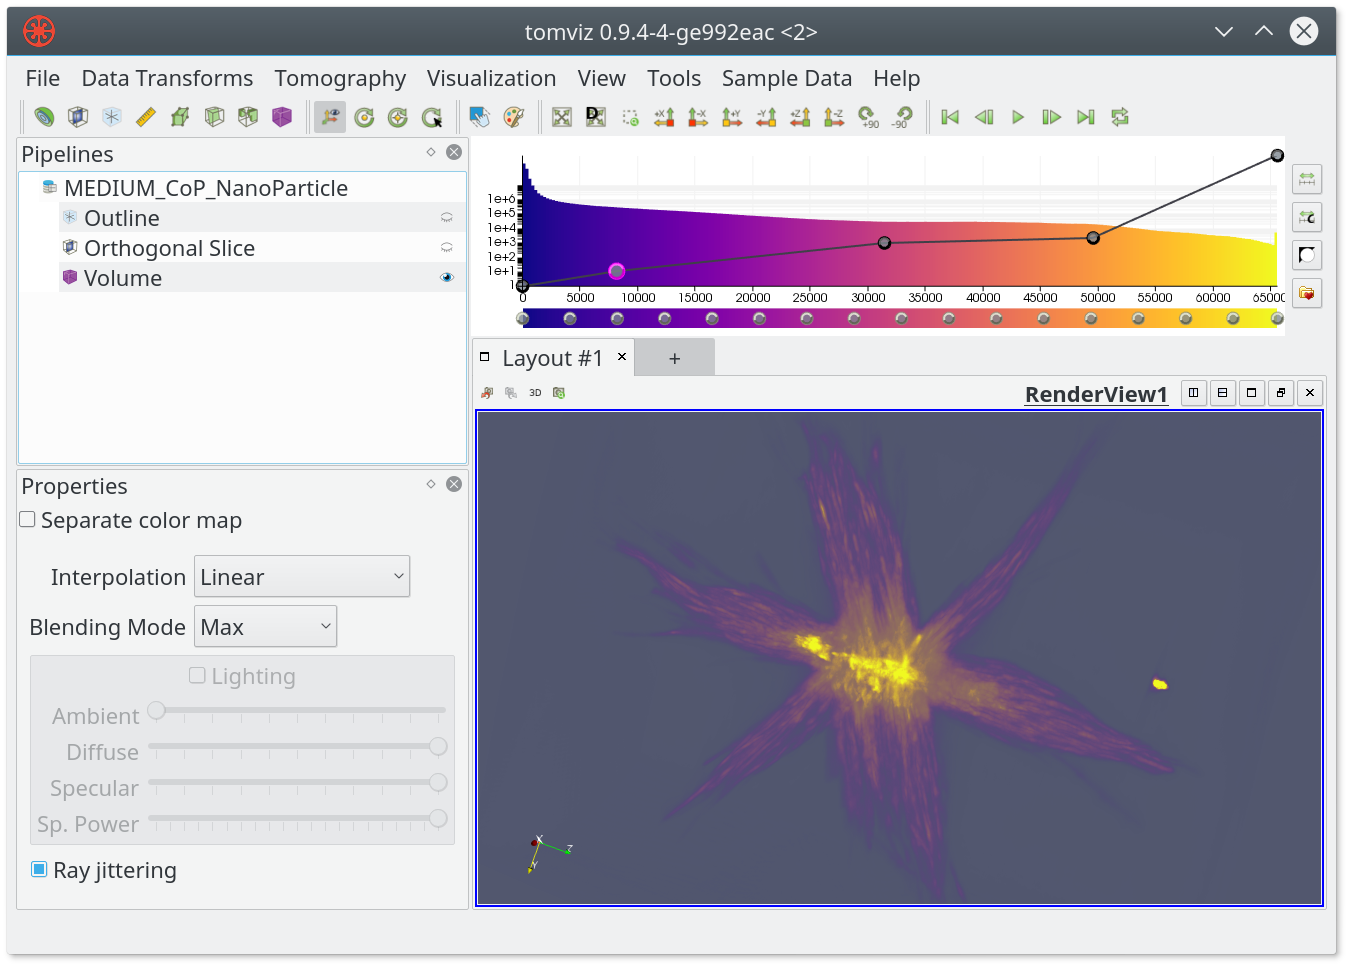
\includegraphics[width=\columnwidth]{tomviz-medium-CoP.png}
  \caption{Tomviz\protect\cite{marcus_hanwell_tomviz_2014} rendering a
  Cobalt-Phosphorous nanoparticle}
  \label{fig:tomviz-cop}
\end{figure}
